\documentclass[compress,xcolor=table]{beamer}

% Packages
\usepackage[english]{babel}
\usepackage[utf8]{inputenc}
\usepackage[T1]{fontenc}
\usepackage{datetime}
\usepackage{multicol}
\usepackage{algorithm,algorithmic}

\usepackage{xstring}

\setbeamertemplate{block begin}
{
  \par\vskip\medskipamount%
  \IfStrEq{\insertblocktitle}{}{}{
      \begin{beamercolorbox}[colsep*=.75ex]{block title}
        \usebeamerfont*{block title}\insertblocktitle%
      \end{beamercolorbox}%
  }
  {\parskip0pt\par}%
  \ifbeamercolorempty[bg]{block title}
  {}
  {\ifbeamercolorempty[bg]{block body}{}{\nointerlineskip\vskip-0.5pt}}%
  \usebeamerfont{block body}%
  \begin{beamercolorbox}[colsep*=.75ex,vmode]{block body}%
    \ifbeamercolorempty[bg]{block body}{\vskip-.25ex}{\vskip-.75ex}\vbox{}%
}



% Possible options of the package (add/remove below in \usetheme call):
%  - nosectionpages: no pages between sections
%  - flama: use flama font, requires xelatex/lualatex + the font to compile
%  - compressminiframes: put the heading list bullets indications pages on 1 line
\usetheme[compressminiframes]{sorbonne}

% Title page
\title{\LARGE Dynamic Adaptation in \\Stream Processing Systems}
\foottitle{D. Wladdimiro}
%\subtitle{PhD Defense} % optional subtitle
\date{Paris - France\\8 January 2023}
\author{Daniel WLADDIMIRO\\
{\footnotesize Directeur de thèse : Pierre SENS\\
Co-encadrants : Luciana ARANTES et Nicolas HIDALGO}}
\institute{LIP6 - Sorbonne Université, CNRS}



% Biblatex
\usepackage[backend=bibtex, style=authoryear, citestyle=authoryear]{biblatex}
\bibliography{library.bib}
\renewcommand*{\bibfont}{\footnotesize}


\begin{document}

\begin{frame}[plain]
	\titlepage
	\setcounter{framenumber}{0}
\end{frame}

\begin{frame}{Table of contents}
\tableofcontents
\end{frame}

\section[1]{Introduction}

\begin{frame}{Context}
	Web 2.0
		\begin{itemize}
			\item High data volumes
			\item Dynamic behaviour of the data flow
		\end{itemize}
	
	\begin{figure}
    	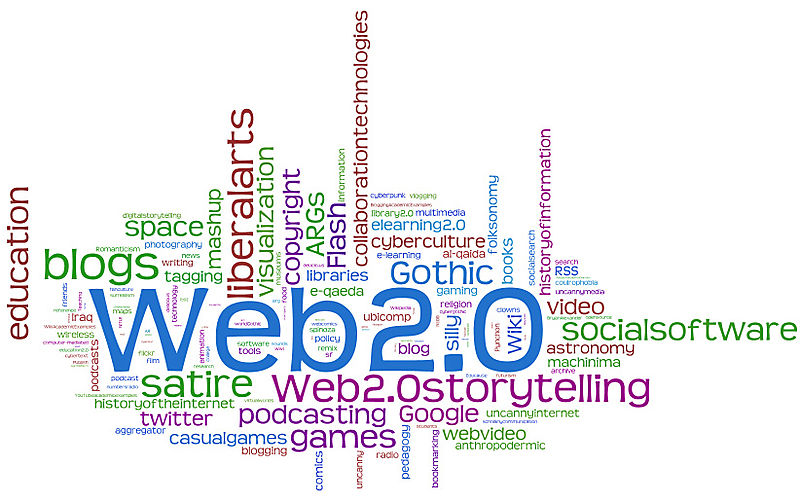
\includegraphics[width=0.6\textwidth]{images/problems/Web.jpg}
    \end{figure}
\end{frame}

\begin{frame}{Context}
		\begin{itemize}
			\item Real-time processing of large data streams
			\begin{itemize}
				\item Low-latency processing
			\end{itemize}
		\end{itemize}
	
		Applications
		\begin{itemize}
			\item Stock exchange prediction
			\item Network security monitoring
			\item Collecting information in natural disasters
		\end{itemize}
\end{frame}

\begin{frame}{Stream processing systems (SPS)}
	Logical architecture
		\begin{itemize}
    		\item The DAG defines the processing logic of the SPS
    		\item A vertex represents a processing operator
    		\item Unidirectional edges represent the data flow
		\end{itemize}
    
    \begin{figure}
		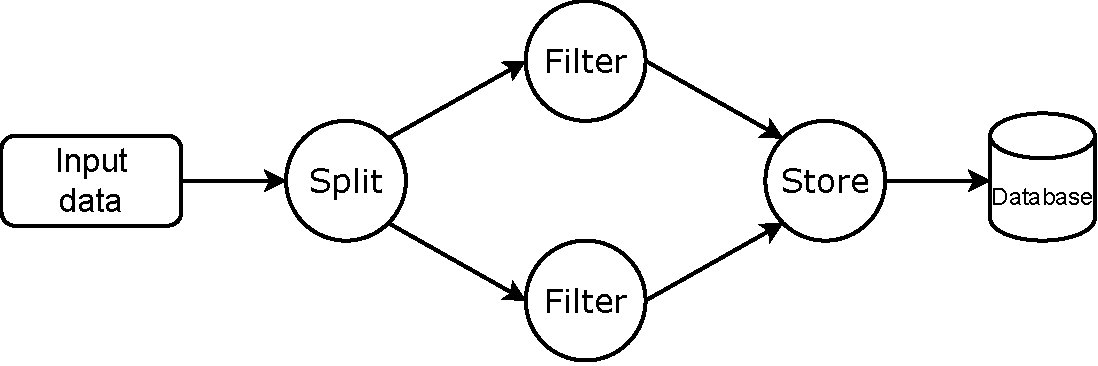
\includegraphics[width=0.75\textwidth]{images/problems/SPS-Concept.pdf}
	\end{figure}
\end{frame}

\begin{frame}{Stream processing systems (SPS)}
	Physical architecture
		\begin{itemize}
    		\item The DAG  must be mapped to a physical environment
    		\item Distributed platform : Cluster or Cloud
		\end{itemize}
	
	\begin{figure}
		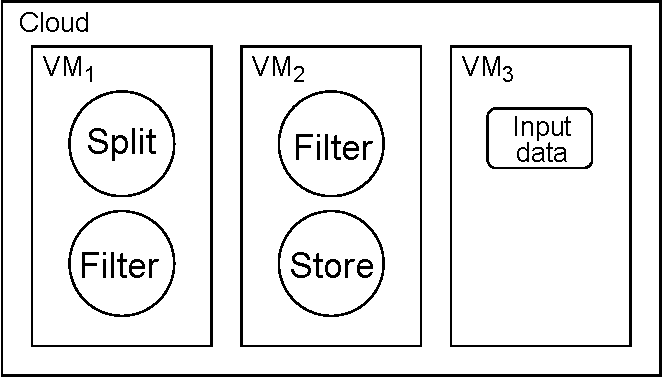
\includegraphics[width=0.5\textwidth]{images/problems/SPS-Physical.pdf}
	\end{figure}
\end{frame}

\begin{frame}{Existing SPS}
	Input rate can present traffic spikes or peaks

	\begin{figure}
		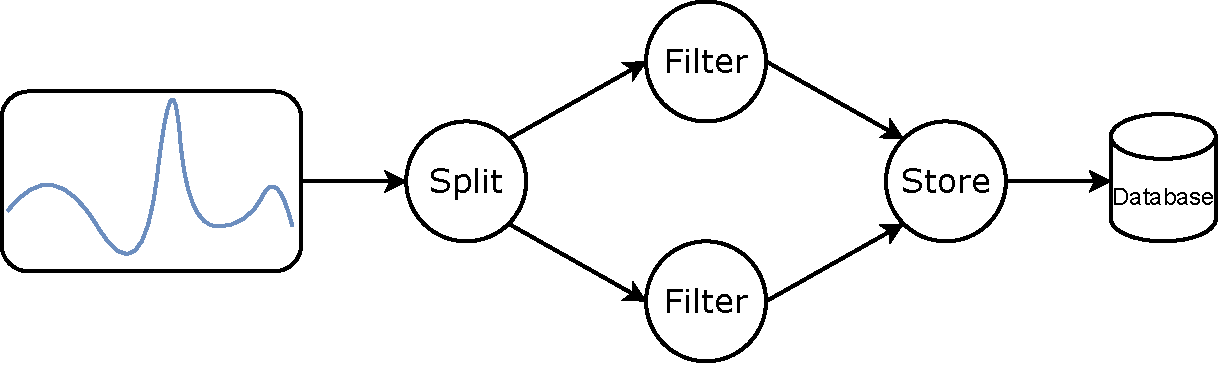
\includegraphics[width=0.65\textwidth]{images/problems/SPS-DynamicDataFlow.pdf}
	\end{figure}
	
	\pause
	
	\begin{alertblock}{Situation}
 	 Overloaded operators and increased end-to-end latency
	\end{alertblock}
\end{frame}

\begin{frame}{Existing SPS}
	Existing SPS Frameworks: 
	\begin{itemize}
		\item Apache Storm [\cite{toshniwal2014storm}]
   		\item Apache Flink [\cite{CarboneKEMHT15}]
	\end{itemize}
    
    \begin{figure}
		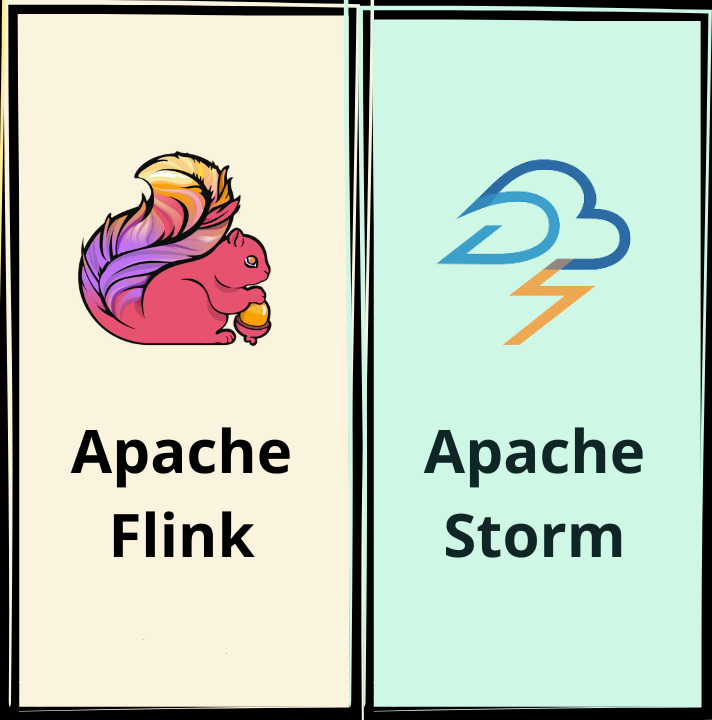
\includegraphics[width=0.4\textwidth]{images/problems/SPS-Framework.png}
	\end{figure}
\end{frame}

\begin{frame}{Existing SPS}
	Replication : Operators can be parallelised
   
    \begin{figure}
		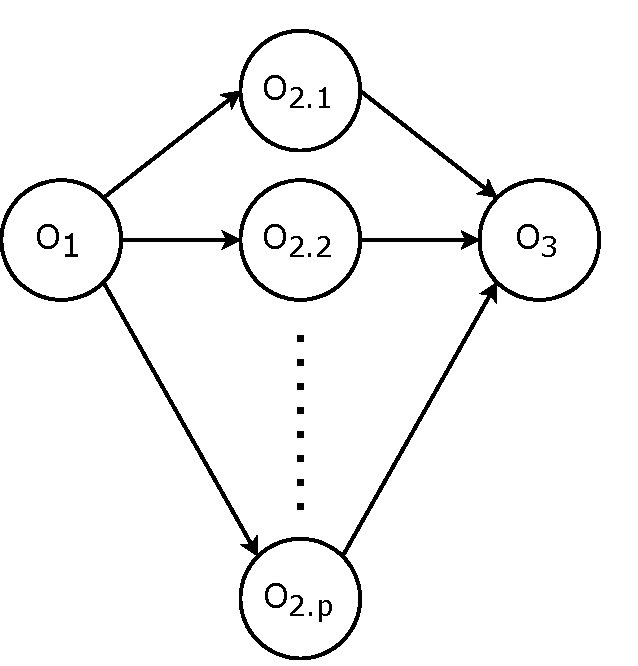
\includegraphics[width=0.35\textwidth]{images/problems/SPS-Operator-Parallelism-Logical.pdf}
	\end{figure}
	
	\pause
	
	\begin{alertblock}{Situation}
		Overprovisioning or underprovisioning of replicas
	\end{alertblock}
\end{frame}



\begin{frame}{Existing SPS}
	\begin{alertblock}{Problem}
		\begin{itemize}
			%\item In general, SPS can present significant fluctuation (peak) in input rate.
		    \item Majority SPSs do not dynamically adapt the number of replicas according to input rate
		\end{itemize}
	\end{alertblock}
	\pause
	\begin{block}{Solution}
		Automatically increase/decrease the number of replicas of critical operators
	\end{block}
\end{frame}

\section[2]{Existing Adaptive SPS}
\begin{frame}{Existing Adaptive SPS}
	Adaptive SPS can modify the number of replicas
	
	\begin{figure}
		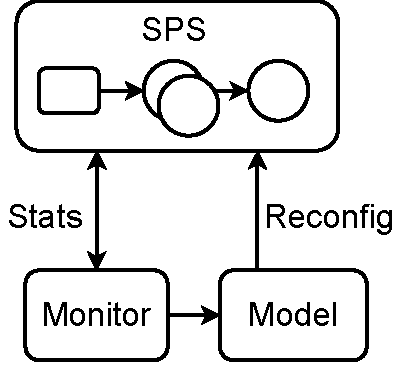
\includegraphics[scale=0.5]{images/concepts/RW-Automatic.pdf}
	\end{figure}
	
	There are two approaches:
	\begin{itemize}
		\item Reactive approach
		\item Predictive approach
	\end{itemize}
\end{frame}

\begin{frame}{Reactive approach}
	\begin{itemize}
		\item Statistics via a monitor
		\item Operator state analysis using thresholds
	\end{itemize}
	
	\begin{figure}
		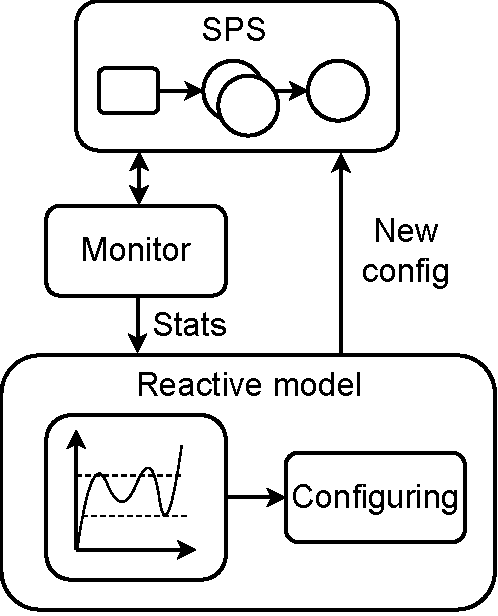
\includegraphics[scale=0.45]{images/concepts/RW-Reactive.pdf}
	\end{figure}
\end{frame}

\begin{frame}{Reactive approach}
	Metrics:
	
	\begin{itemize}
		\item CPU [\cite{GulisanoJPSV12}]
		\item Latency [\cite{MadsenZS16, SatzgerHLD11, HeinzeJHF14}]
		\item Throughput [\cite{KahveciG20, RussoCCP21, GedikSHW14}]
	\end{itemize}
	
	\pause
	
	\begin{alertblock}{Limitation}
		Most solutions consider a single metric
	\end{alertblock}
\end{frame}

\begin{frame}{Predictive approach}
	\begin{itemize}
		\item Based on prediction to determine the SPS reconfiguration
		\item Apply a predictor model
	\end{itemize}
	
	\begin{figure}
		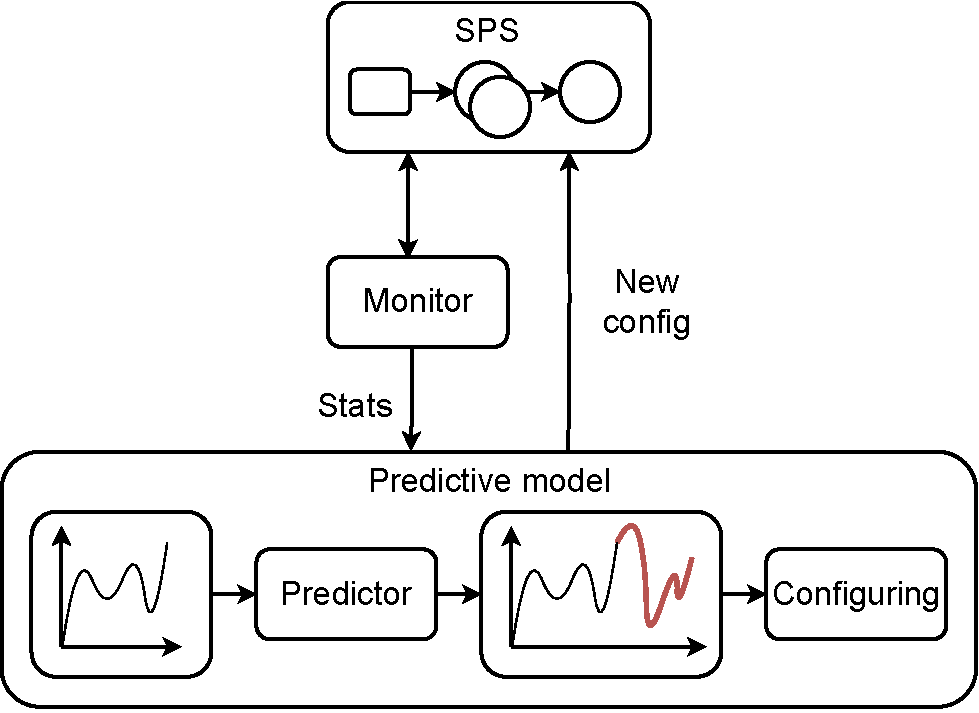
\includegraphics[scale=0.45]{images/concepts/RW-Predictive.pdf}
	\end{figure}
\end{frame}

\begin{frame}{Related Work}
	Predictor models:
	
	\begin{itemize}
		\item Reinforcement learning [\cite{CardelliniPNR18}]
		\item Time series [\cite{KombiLLRB19}]
		\item Fuzzy logic [\cite{MencagliTD18}]
		\item ANN [\cite{LombardiABQ18}]
	\end{itemize}
	
	\pause
	
	\begin{alertblock}{Limitation}
		Predictive models are specific to an input rate or scenario
	\end{alertblock}
\end{frame}






\section[3]{Our Adaptive SPS}

\begin{frame}{Our Adaptive SPS}
	\begin{exampleblock}{Our Proposal}
		An adaptive SPS based on \textbf{MAPE model} whose aim is to \textbf{adapt the number of replicas} of the operators according to the peaks in the data stream.
	\end{exampleblock}
	
	\only<1>{
	\begin{figure}
		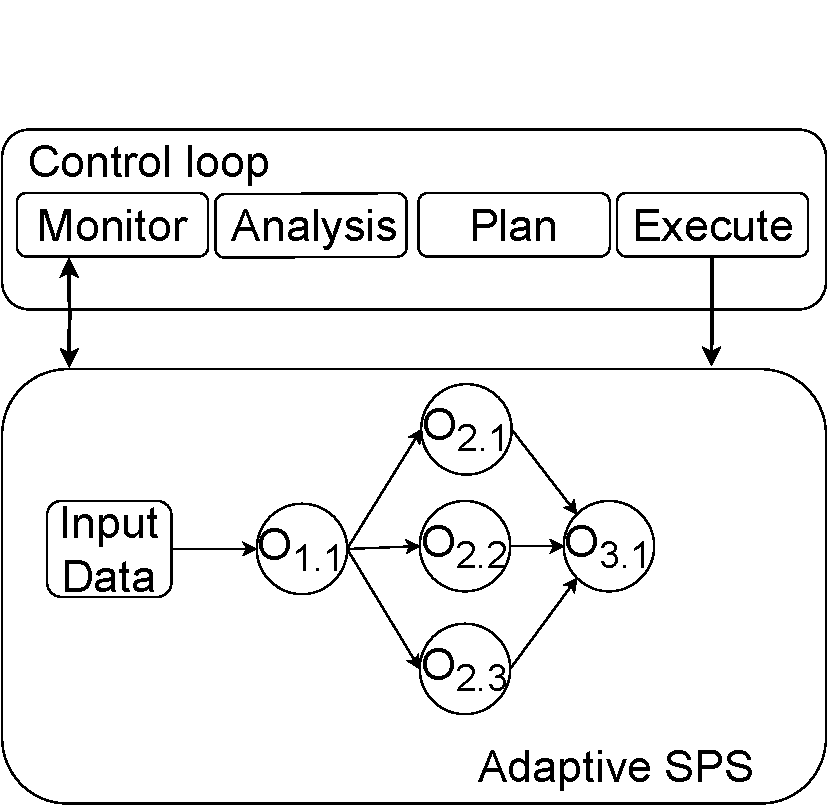
\includegraphics[scale=0.35]{images/problems/SPS-MAPE.pdf}
	\end{figure}
	}
	
	\only<2>{
	\begin{figure}
		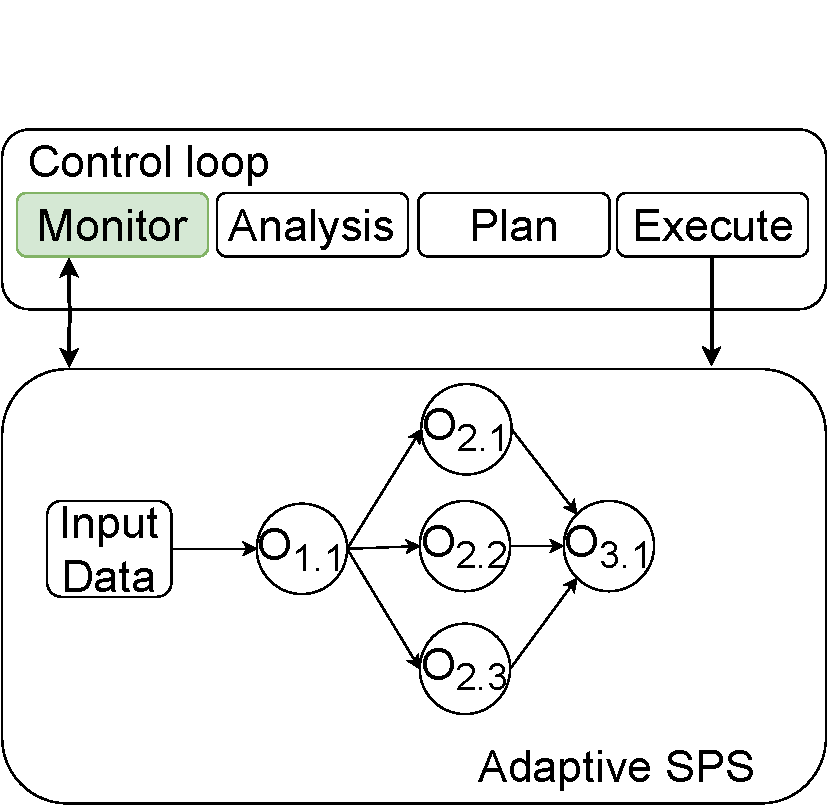
\includegraphics[scale=0.35]{images/problems/SPS-MAPE-M.pdf}
	\end{figure}
	}
	
	\only<3>{
	\begin{figure}
		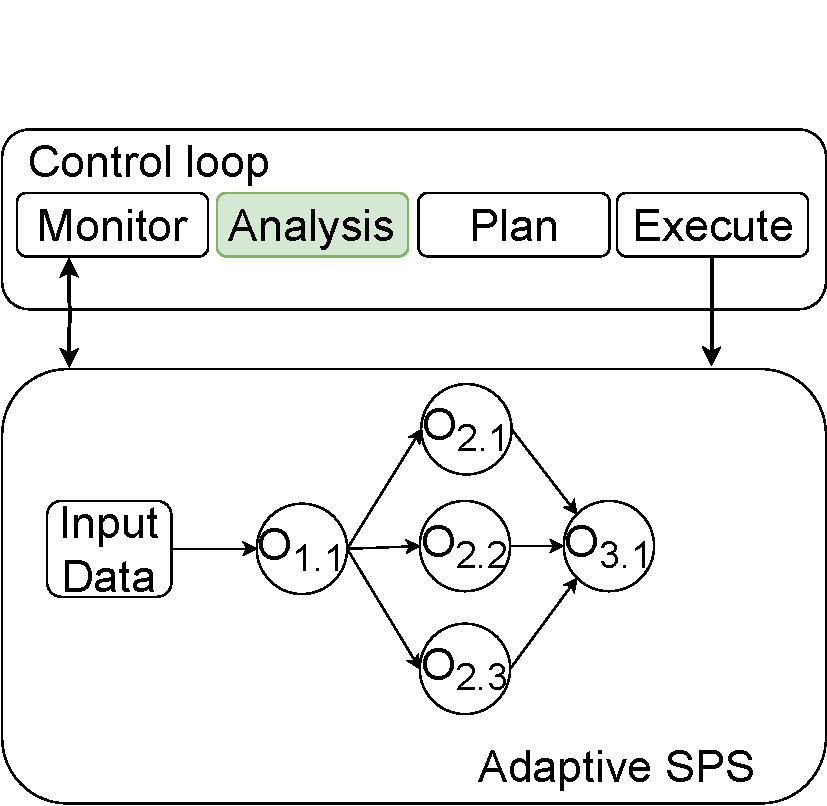
\includegraphics[scale=0.35]{images/problems/SPS-MAPE-A.pdf}
	\end{figure}
	}
	
	\only<4>{
	\begin{figure}
		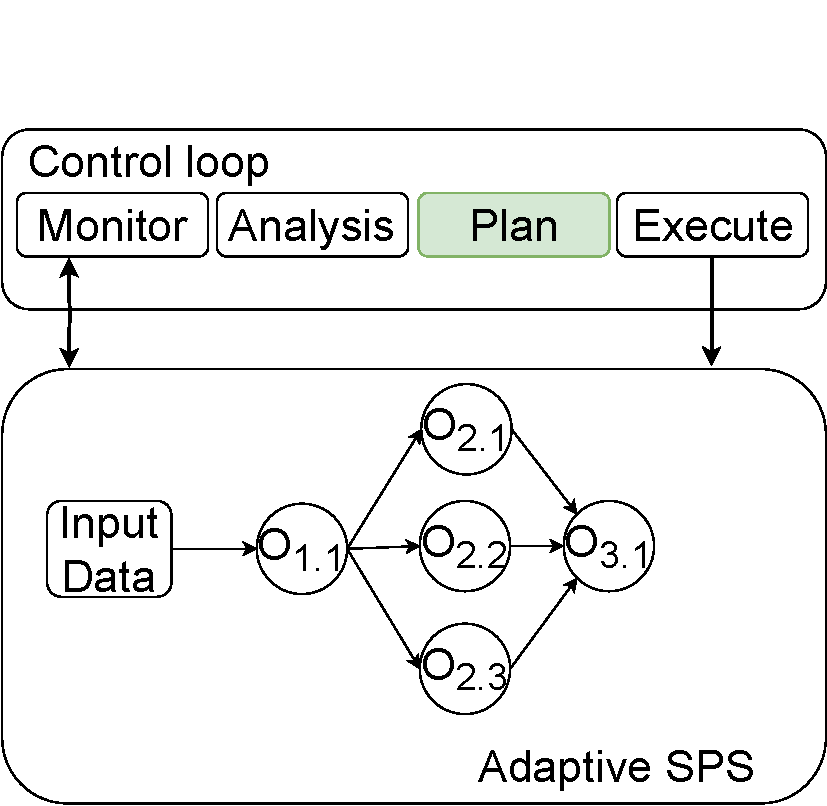
\includegraphics[scale=0.35]{images/problems/SPS-MAPE-P.pdf}
	\end{figure}
	}
	
	\only<5>{
	\begin{figure}
		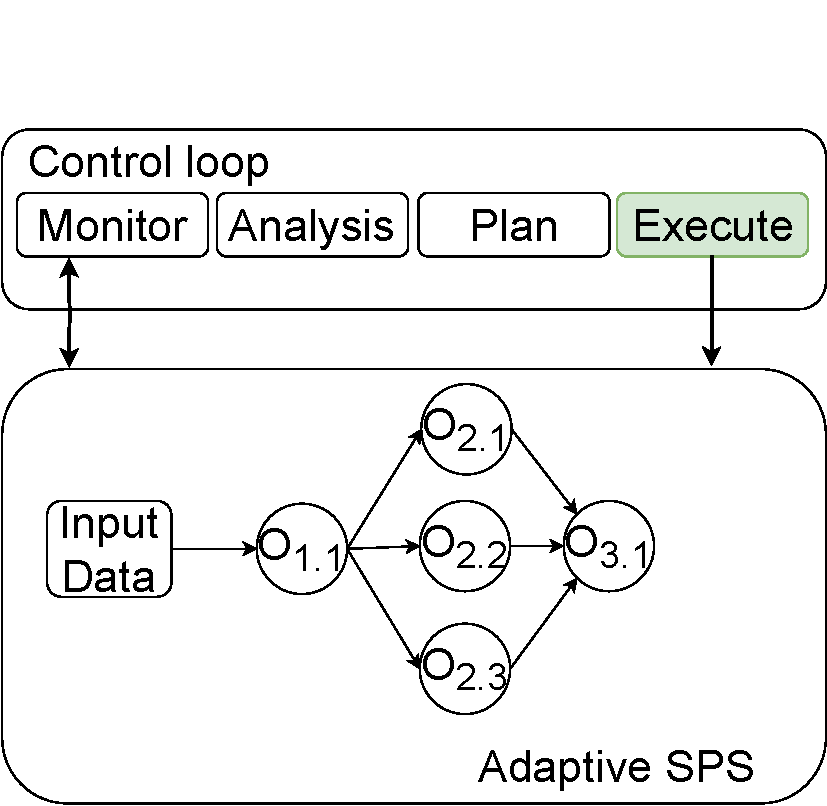
\includegraphics[scale=0.35]{images/problems/SPS-MAPE-E.pdf}
	\end{figure}
	}
\end{frame}

\begin{frame}{Our Adaptive SPS}
	Present two approaches:
	\begin{itemize}
		\item \textbf{Reactive approach} (RA-SPS): on-the-fly analysis of operator load
		\item \textbf{Predictive approach} (PA-SPS): predicting the number of replicas required
	\end{itemize}
\end{frame}

\begin{frame}{Our Adaptive SPS : Implementation}	
	An extension of Apache Storm	
		
	\begin{figure}
		
\includegraphics[scale=0.15]{images/concepts/Storm.png}
	\end{figure}
\end{frame}	

\begin{frame}{Storm limitation}	
	\begin{alertblock}{Limitation}
		Downtime in each reconfiguration	
	\end{alertblock}
	
	\begin{figure}
		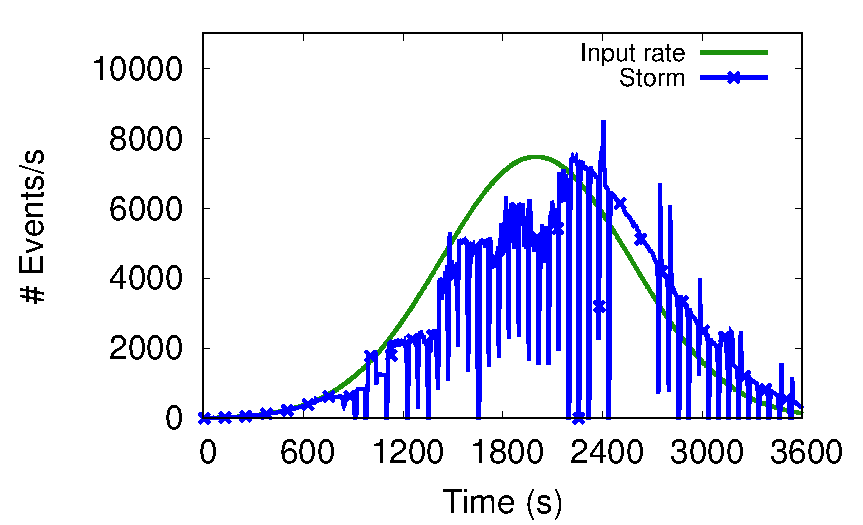
\includegraphics[scale=0.5]{images/problems/Pool.pdf}
	\end{figure}	
\end{frame}

\begin{frame}{Our Adaptive SPS : Pool of replicas}
	Pool of pre-allocate replicas for each operator.
	
	\only<1>{
	\begin{figure}
		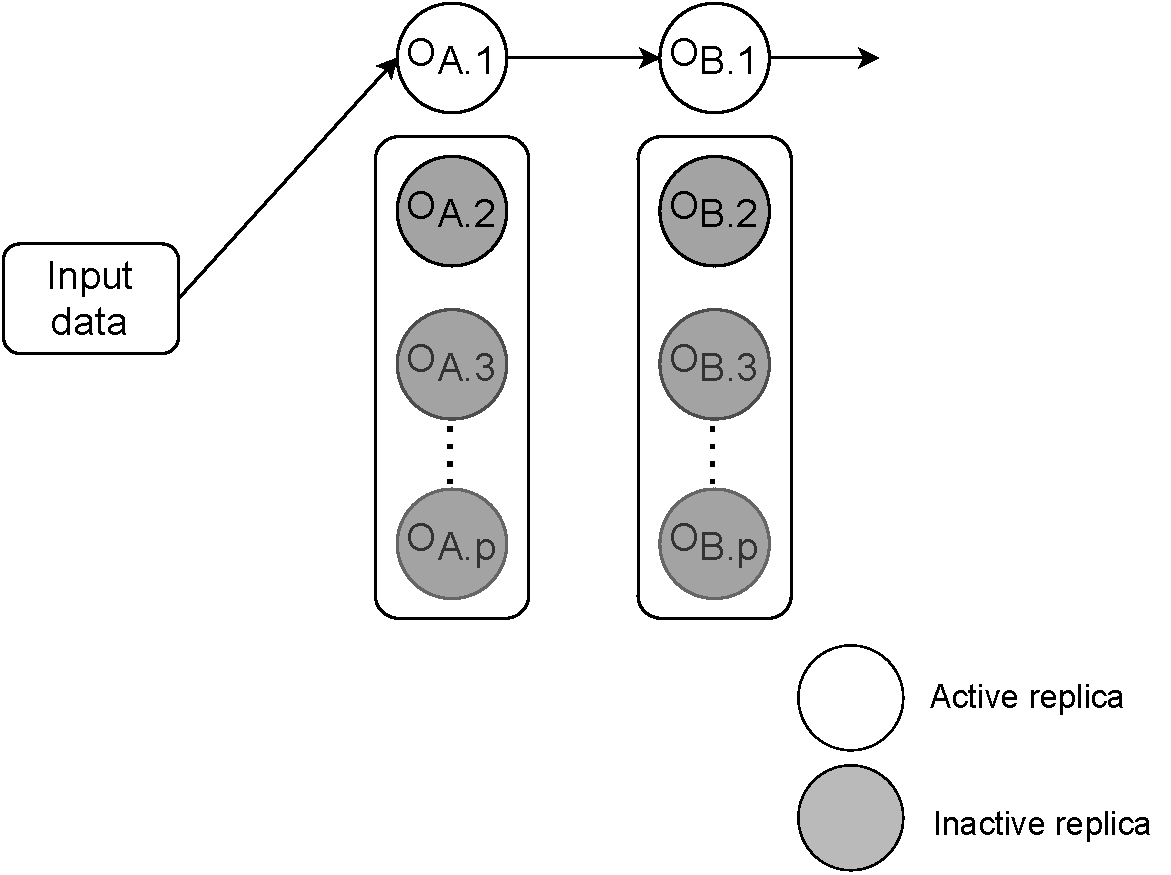
\includegraphics[width=0.75\textwidth]{images/problems/PoolReplicas1.pdf}
	\end{figure}
	}

	\only<2>{
	\begin{figure}
		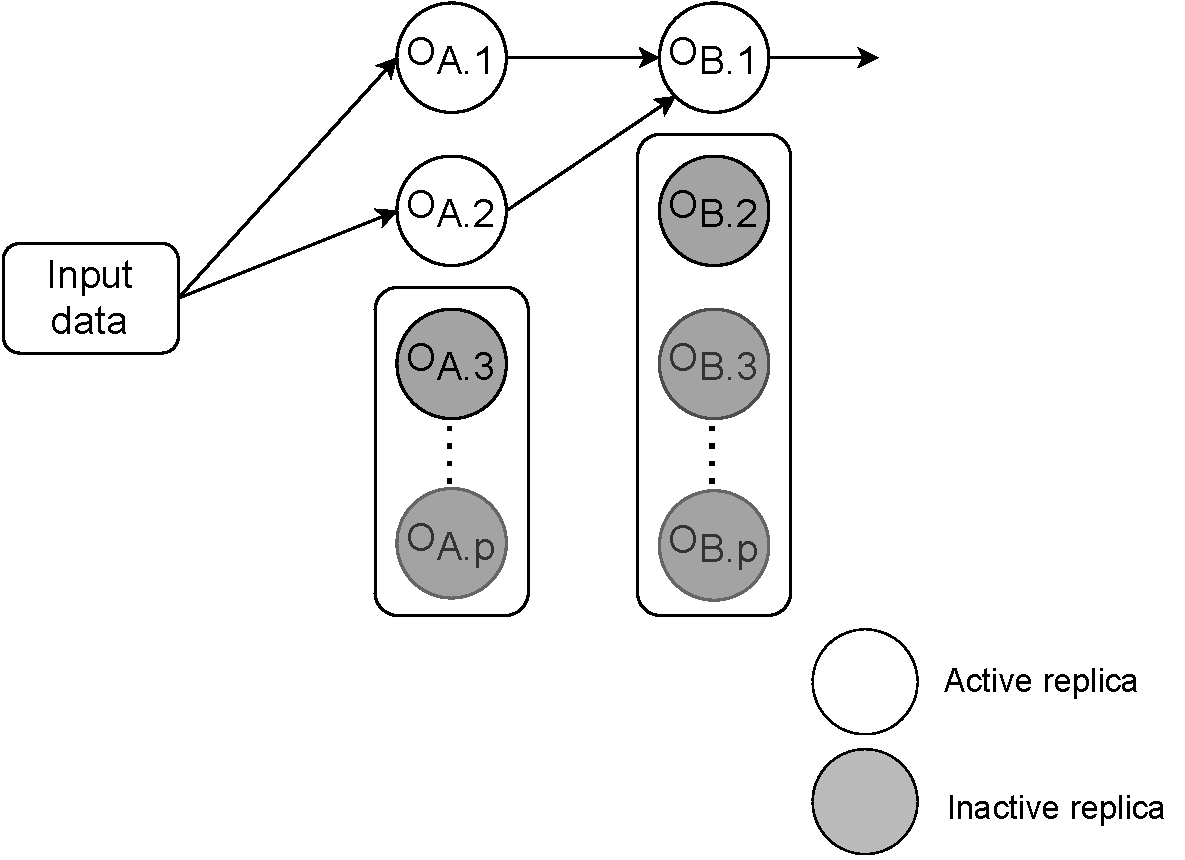
\includegraphics[width=0.75\textwidth]{images/problems/PoolReplicas2.pdf}
	\end{figure}
	}
\end{frame}

\begin{frame}{Storm limitation}
	
	\only<1>{
		Shuffle grouping (Round-robin) among the active replicas of an operator
	\begin{figure}
		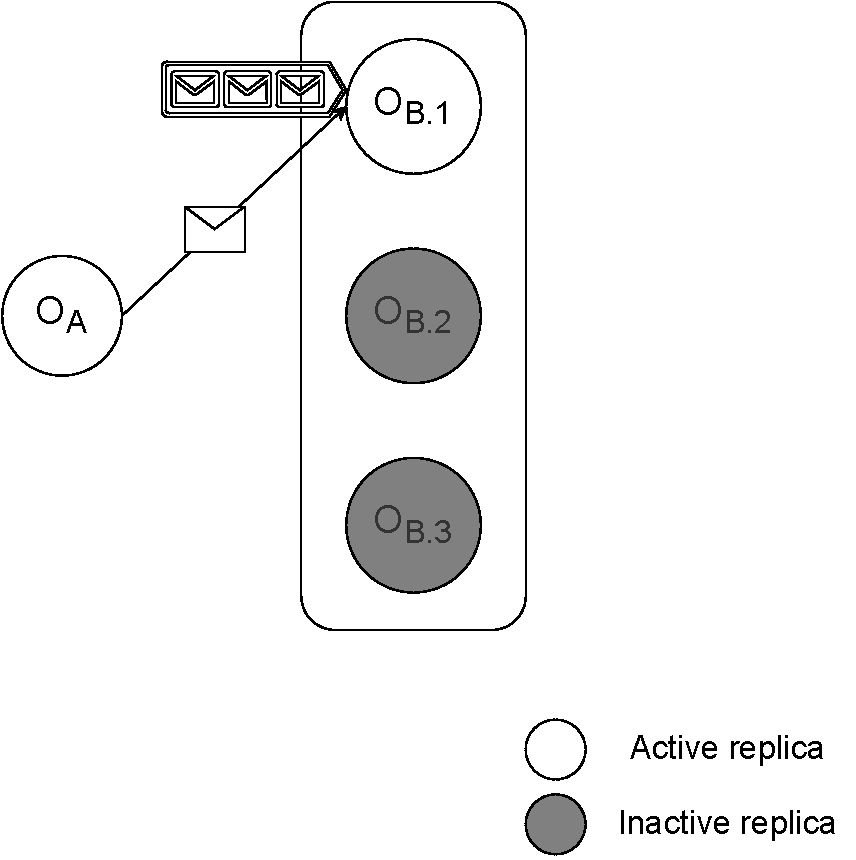
\includegraphics[width=0.62\textwidth]{images/problems/LoadGrouping.pdf}
	\end{figure}
	}

	\only<2>{
	\begin{alertblock}{Limitation}
		Load balancing among active replicas
	\end{alertblock}	
	
	\begin{figure}
		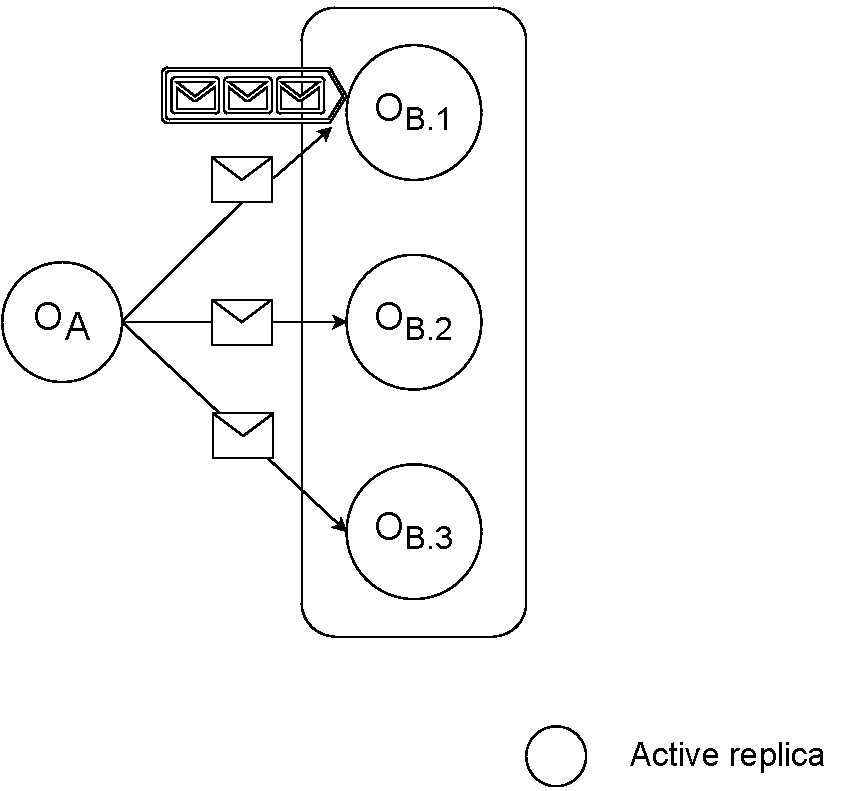
\includegraphics[width=0.64\textwidth]{images/problems/LoadGrouping1.pdf}
	\end{figure}
	}
\end{frame}
	
\begin{frame}{Our Adaptive SPS : Load-Aware grouping}
	Stream grouping for distributing the load among the active replicas of an operator
	\begin{figure}
		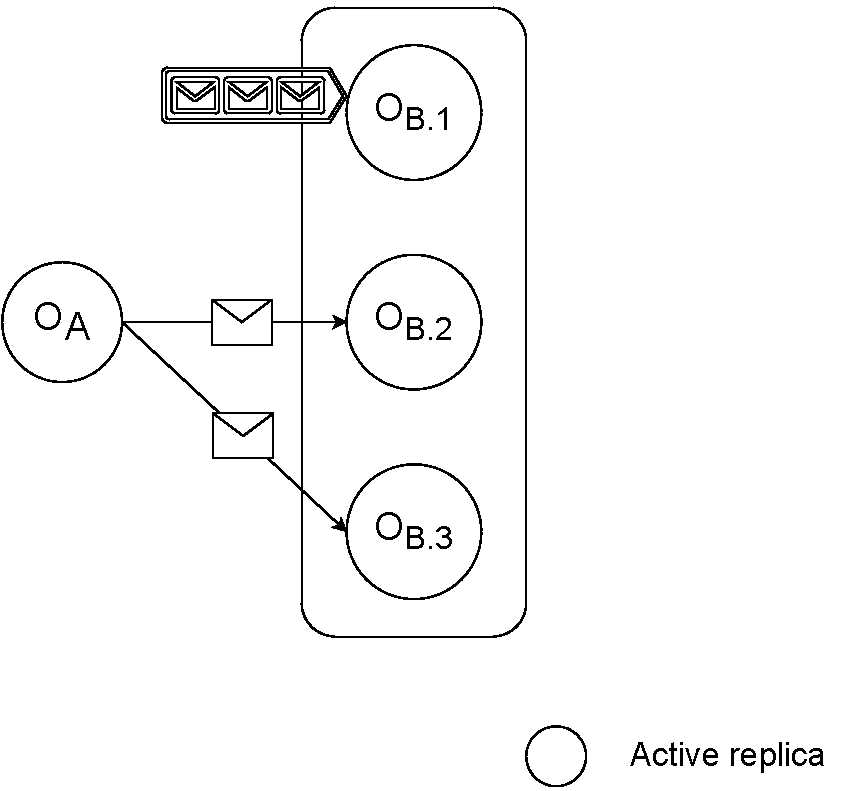
\includegraphics[width=0.65\textwidth]{images/problems/LoadGrouping2.pdf}
	\end{figure}
\end{frame}






\begin{frame}[noframenumbering]
	\centering
	\huge Our Adaptive SPS \\ Reactive approach (RA-SPS)
\end{frame}


\begin{frame}{Reactive approach : RA-SPS}
	\begin{block}{Proposal}
	Analyse the \textbf{operator state} to modify the number of active replicas of the operators in the DAG		
	\end{block}
\end{frame}

\begin{frame}{Reactive approach : RA-SPS}
	State metric $\delta$ is a multi-metric based in : 
	\begin{itemize}
		\item Utilization (U) : Operator load
		\item Execution time (E) : Degradation execution time
		\item Queue (Q) : Impact of queue size
	\end{itemize}
	\vspace*{0.5cm}	
	Each metric is discrete and calculated according to the time interval $t$
	\vspace*{-2.5cm}
	\begin{figure}
		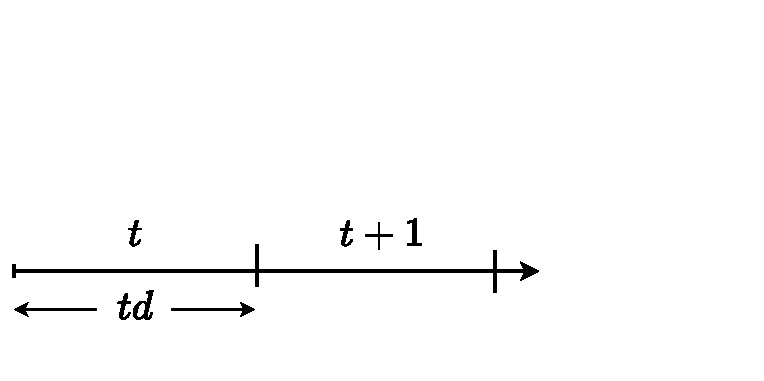
\includegraphics[scale=0.75]{images/concepts/Interval.pdf}
	\end{figure}
\end{frame}

\begin{frame}{Reactive approach : RA-SPS}
	\textbf{Utilisation metric}\\
	\vspace*{0.2cm}
	Percentage of time that the operator $O_i$ is processing during $t$
	\begin{align*}
        U_i(t) = \frac{\mu_i(t) \times et_i(t)}{r_i(t) \times td}
   	\end{align*}   	
%   	\begin{tabular}{r l}
%   	$\mu_i(t)$ & number of events processed by operator $O_i$ during $t$ \\
%   	${et}_i(t)$ & average execution of one event by operator $O_i$ during $t$ \\
%	$r_i(t)$ & number of active replicas of operator $O_i$ during $t$ \\
%	$td$ & time interval duration \\
%   	\end{tabular}
\end{frame}

\begin{frame}{Reactive approach : RA-SPS}
	\textbf{Utilisation metric}
	\begin{center}
	\begin{align*}
        U_i(t) = \frac{\mu_i(t) \times et_i(t)}{r_i(t) \times td}
   	\end{align*}
   	\vspace*{-1cm}
   	\begin{figure}
   		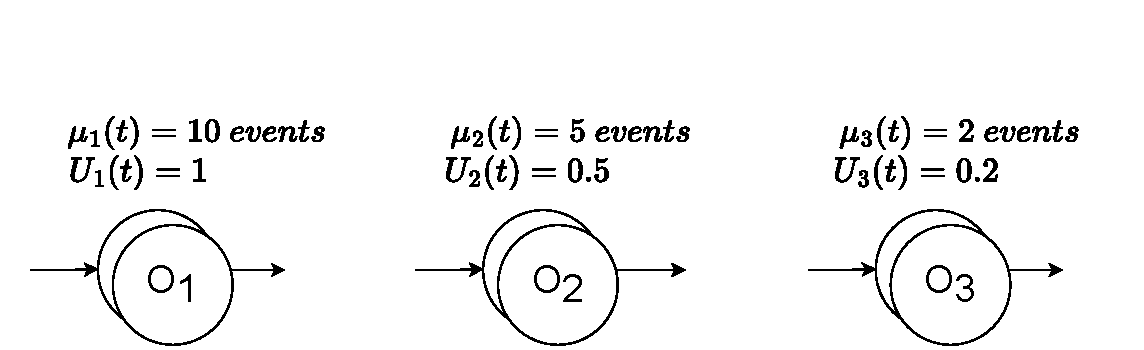
\includegraphics[scale=0.5]{images/concepts/reactive/RA-SPS-Metric-U.pdf}
   	\end{figure}
 	
  	$et_i(t) = 200~ms$ ; $r_i(t) = 2~ms$ ; $td = 1000~ms$ ; $i \in [1,2,3]$
  	\end{center}
\end{frame}
   	
\begin{frame}{Reactive approach : RA-SPS}
	\textbf{Execution time metric}\\
	\vspace*{0.2cm}
	Execution time degradation of the operator $O_i$ during $t$
%	\begin{center}	
   	\begin{align*}
        E_i(t) = 1-\frac{et_i}{et_i(t)}
    \end{align*}
    \vspace*{0.2cm}
    
    \begin{tabular}{r l}
%   	${et}_i(t)$ & average execution of one event by operator $O_i$ during $t$ \\
	${et}_i$ & average execution time of one event by operator $O_i$ \\
	 		 & according to the benchmark\\
   	\end{tabular}
%   	\end{center}
\end{frame}

\begin{frame}{Reactive approach : RA-SPS}
	\textbf{Execution time metric}
	\begin{center}
	\begin{align*}
        E_i(t) = 1-\frac{et_i}{et_i(t)}
   	\end{align*}
   	\vspace*{-0.75cm}
   	\begin{figure}
   		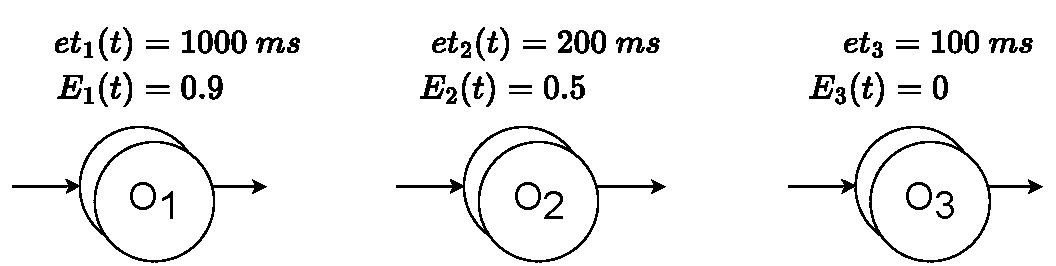
\includegraphics[scale=0.5]{images/concepts/reactive/RA-SPS-Metric-E.pdf}
   	\end{figure}
 	
  	$et_i = 100~ms$ ; $i \in [1,2,3]$
  	\end{center}
\end{frame}
    
\begin{frame}{Reactive approach : RA-SPS}    
	\textbf{Queue metric}\\
	\vspace*{0.2cm}
	Impact of the queue size of the operator $O_i$ according to the processing during $t$
%	\begin{center}
    \begin{align*}
        Q_i(t) = 1-\frac{\mu_i(t)}{q_i(t)}
    \end{align*}
    
%    \begin{tabular}{r l}
%   	$\mu_i(t)$ & number of events processed by operator $O_i$ during $t$ \\
%	$q_i(t)$ & number of events queued by operator $O_i$ during $t$ \\
%   	\end{tabular}
%   	\end{center}
\end{frame}

\begin{frame}{Reactive approach : RA-SPS}
	\textbf{Queue metric}
	\begin{center}
	\begin{align*}
        Q_i(t) = 1-\frac{\mu_i(t)}{q_i(t)}
   	\end{align*}
   	\vspace*{-0.75cm}
   	\begin{figure}
   		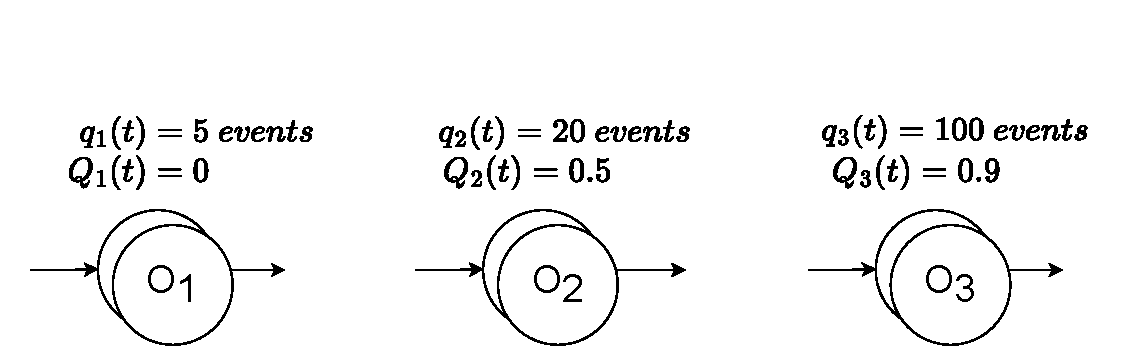
\includegraphics[scale=0.5]{images/concepts/reactive/RA-SPS-Metric-Q.pdf}
   	\end{figure}
 	
  	$\mu_i(t) = 10~events$ ; $i \in [1,2,3]$
  	\end{center}
\end{frame}
	
\begin{frame}{Reactive approach : RA-SPS}
		\textbf{State metric} $\delta_i(t)$ is determined by the three metrics and their respective weights
        \begin{align*}
            \delta_i(t) = U_i(t) \times \omega_U + Q_i(t) \times \omega_Q + E_i(t) \times \omega_E
        \end{align*}   
\end{frame}
	
\begin{frame}{Reactive approach : RA-SPS}
	Analysis of the operator state
		
		\begin{tabular}{l l}
		$\delta_i(t) < \delta_l$ & underloaded \\
		$\delta_l \leq \delta_i(t) \leq \delta_u$ & stable \\
		$\delta_i(t) > \delta_l$ & overloaded
		\end{tabular}
	
	\begin{figure}
		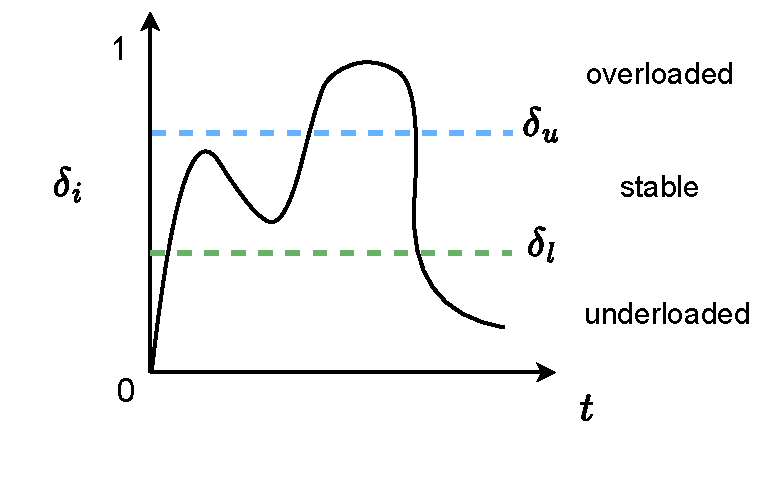
\includegraphics[scale=0.6]{images/concepts/reactive/RA-SPS-Metric-Delta.pdf}
	\end{figure}
\end{frame}

\begin{frame}{Reactive approach : RA-SPS}
    \textbf{Planning algorithm}\\
    \vspace*{0.2cm}
    Analyse if the current state is equal to the precedent state
	\begin{figure}
		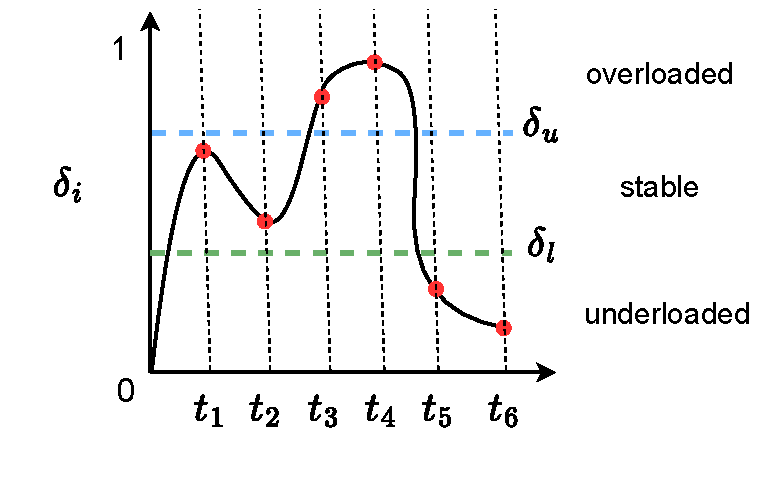
\includegraphics[scale=0.6]{images/concepts/reactive/RA-SPS-Plan.pdf}
	\end{figure}
	\vspace*{-0.2cm}
	\only<1>{
		\textbf{$t_1$}
	}
	
	\only<2>{
		\textbf{$t_2$} : State($\delta_i(t_2)$) $=$ State($\delta_i(t_1)$) ?
	}
	
	\only<3>{
		\textbf{$t_3$} : State($\delta_i(t_3)$) $=$ State($\delta_i(t_2)$) ?
	}
	
	\only<4>{
		
		\textbf{$t_4$} : State($\delta_i(t_4)$) $=$ State($\delta_i(t_3)$) ? Is the machine overloaded ?\\
		 %$E_i(t) > \delta_{E}$ ? \\		
		\textbf{Activate} $k$ replicas of the operator $O_i$
	}
	
	\only<5>{
		\textbf{$t_5$} : State($\delta_i(t_5)$) $=$ State($\delta_i(t_4)$) ?
	}
	
	\only<6>{
		\textbf{$t_6$} : State($\delta_i(t_6)$) $=$ State($\delta_i(t_5)$) ?\\
		\textbf{Deactivate} $k$ replicas of the operator $O_i$
	}
\end{frame}

\begin{frame}[noframenumbering]
	\centering
	\huge Our Adaptive SPS \\ Predictive approach (PA-SPS)
\end{frame}


\begin{frame}{Predictive Approach : PA-SPS}
	\begin{block}{Proposal}
		\textbf{Estimate the number of active replicas} for operator according to the predicted input rate
	\end{block}
\end{frame}

\begin{frame}{Predictive Approach : PA-SPS}
	Predictor model is based in : 
	\begin{itemize}
		\item number of events received
		\item dependency among operators
		\item number of queued events
	\end{itemize}
\end{frame}

\begin{frame}{Predictive Approach : PA-SPS}
\begin{figure}
    \centering
    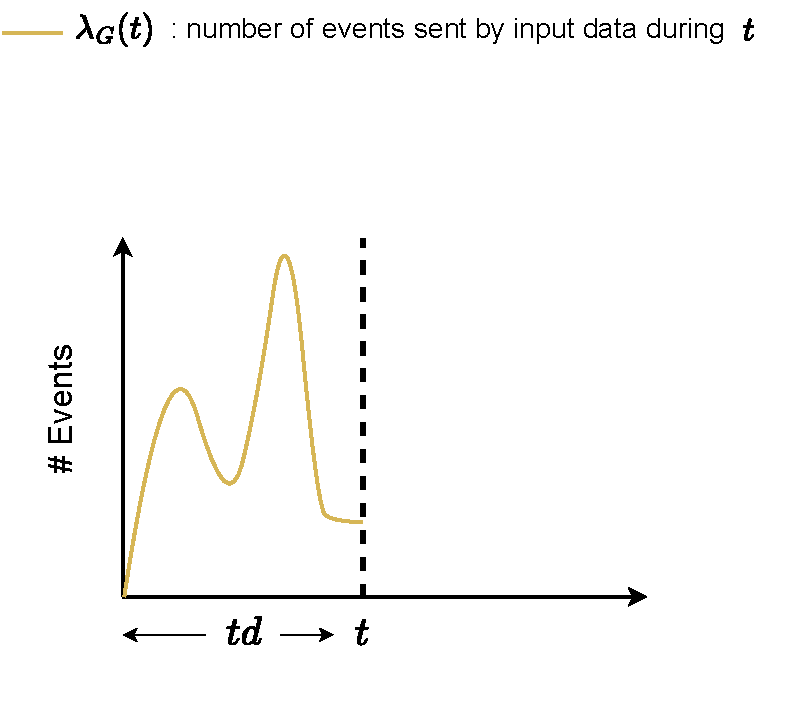
\includegraphics[scale=0.63]{images/concepts/predictive/PA-SPS-Prediction-1.pdf}
\end{figure}
\end{frame}

\begin{frame}{Predictive Approach : PA-SPS}
\begin{figure}
    \centering
    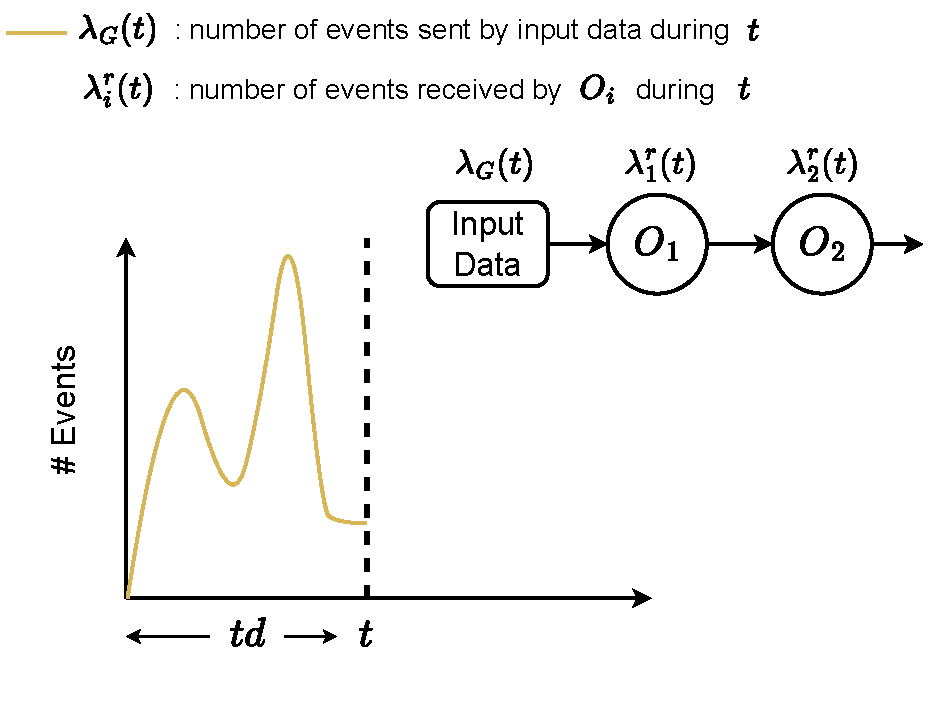
\includegraphics[scale=0.63]{images/concepts/predictive/PA-SPS-Prediction-2.pdf}
\end{figure}
\end{frame}

\begin{frame}{Predictive Approach : PA-SPS}
\begin{figure}
    \centering
    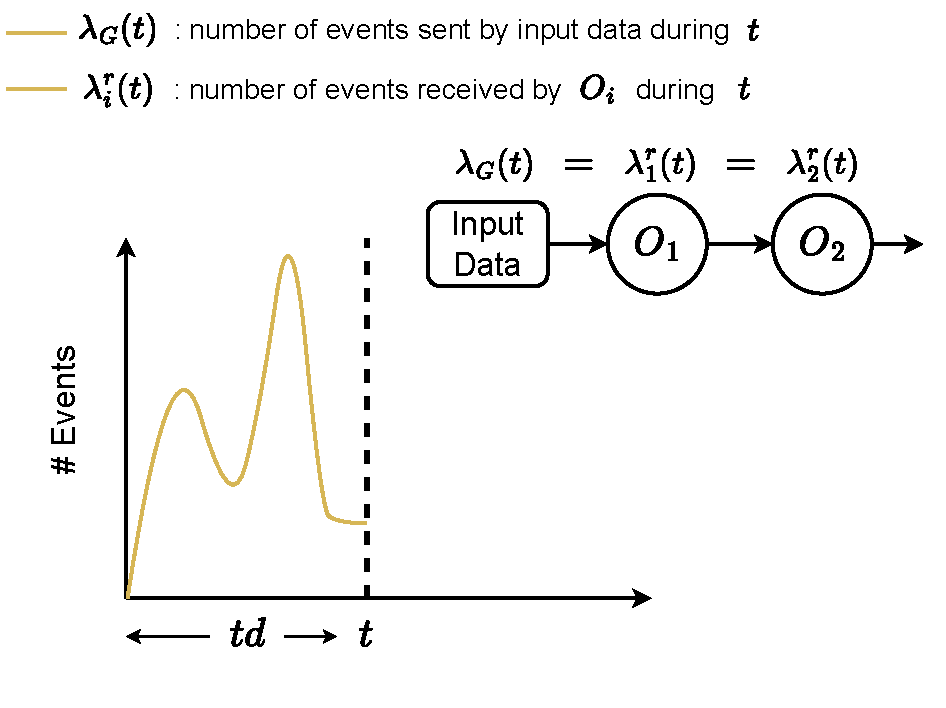
\includegraphics[scale=0.63]{images/concepts/predictive/PA-SPS-Prediction-3.pdf}
\end{figure}
\end{frame}

\begin{frame}{Predictive Approach : PA-SPS}
\begin{figure}
    \centering
    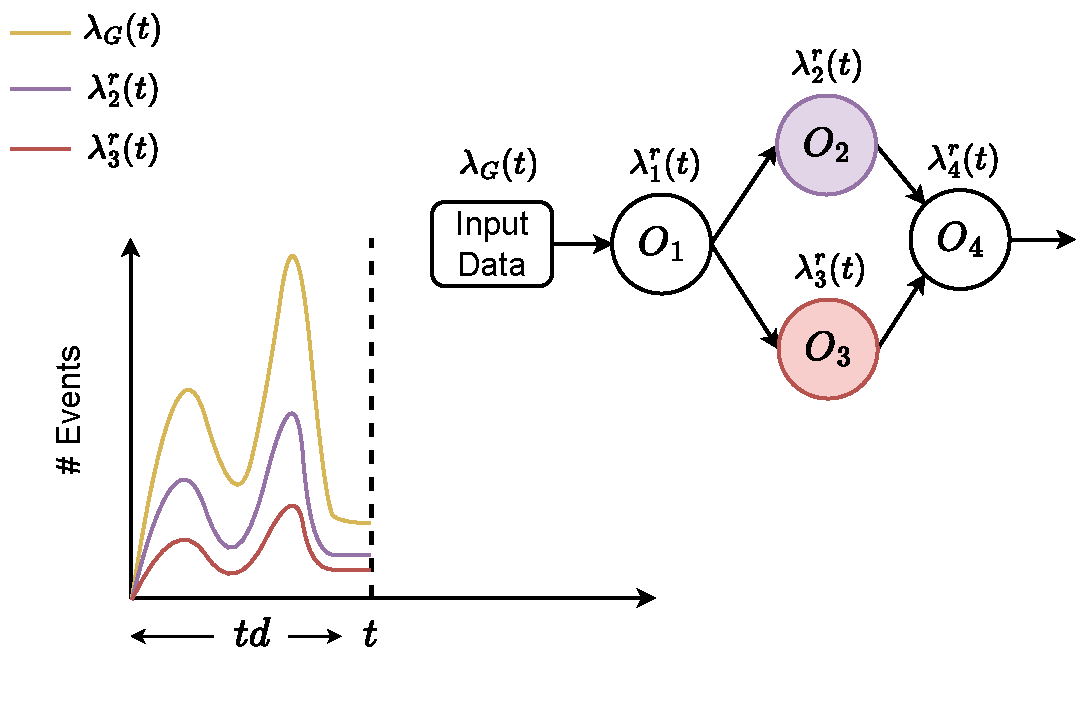
\includegraphics[scale=0.63]{images/concepts/predictive/PA-SPS-Prediction-4.pdf}
\end{figure}
\end{frame}

\begin{frame}{Predictive Approach : PA-SPS}
\vspace*{-0.5cm}
\begin{figure}
    \centering
    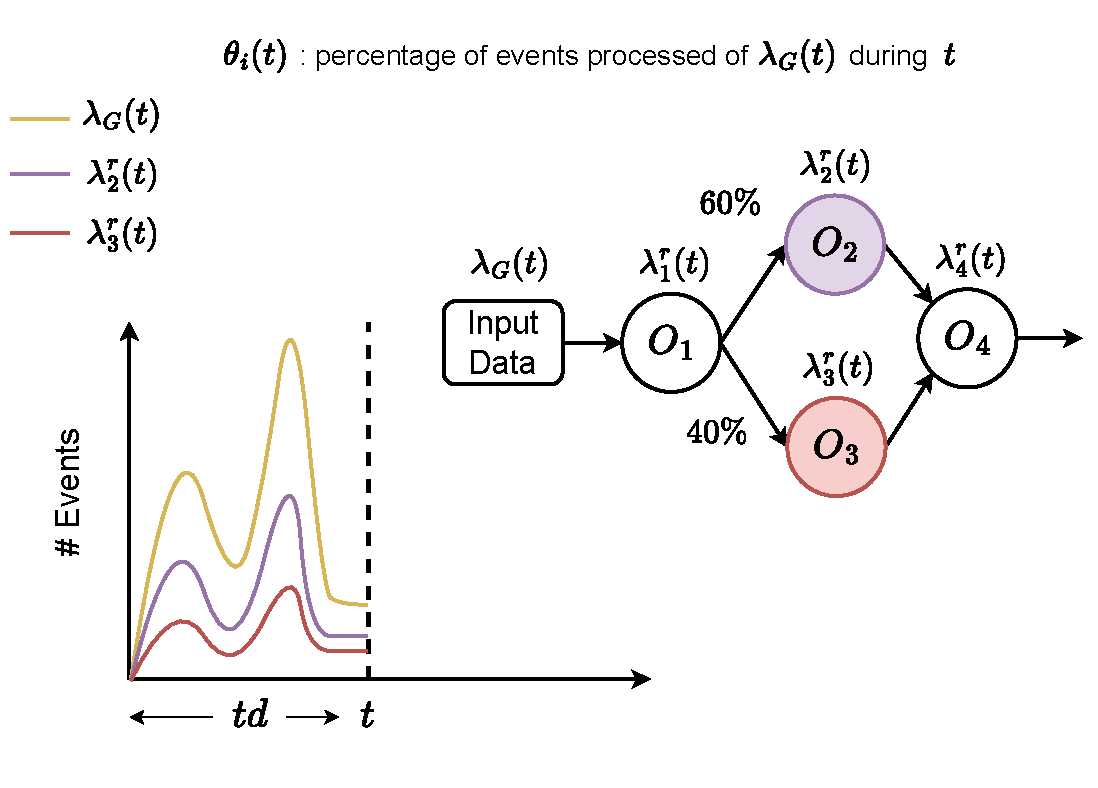
\includegraphics[scale=0.6]{images/concepts/predictive/PA-SPS-Prediction-5.pdf}
\end{figure}
\end{frame}

\begin{frame}{Predictive Approach : PA-SPS}
\begin{figure}
    \centering
    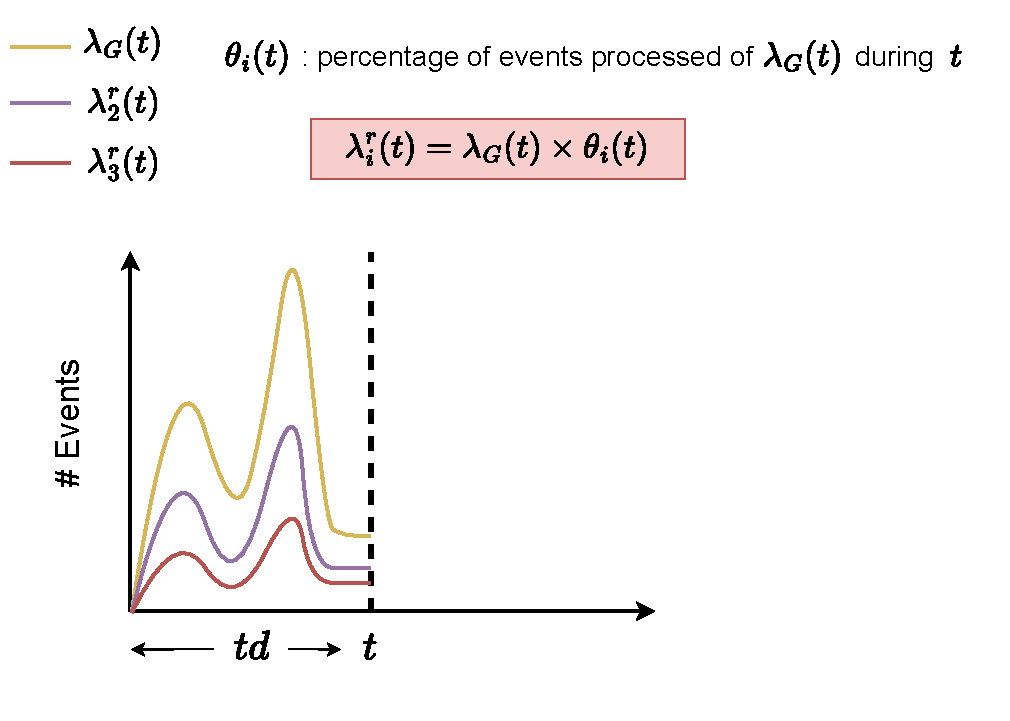
\includegraphics[scale=0.63]{images/concepts/predictive/PA-SPS-Prediction-6.pdf}
\end{figure}
\end{frame}

\begin{frame}{Predictive Approach : PA-SPS}
\begin{figure}
    \centering
    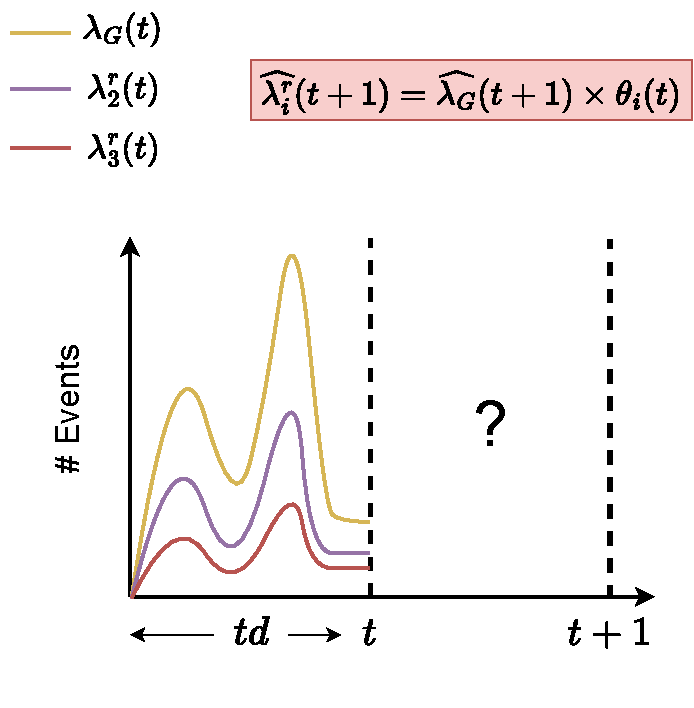
\includegraphics[scale=0.63]{images/concepts/predictive/PA-SPS-Prediction-7.pdf}
\end{figure}
\end{frame}

\begin{frame}{Predictive Approach : PA-SPS}
	\textbf{Predictive model} is used to predict the number of events sent by the input data during the next time interval\\
	\vspace*{0.25cm}
	Predictive models applied:
	\begin{itemize}
		\item Basic
		\item Linear regression
		\item Fast Fourier Transform
		\item Artificial Neural Network
		\item Random Forest
	\end{itemize}

\end{frame}

\begin{frame}{Predictive Approach : PA-SPS}
\begin{figure}
    \centering
    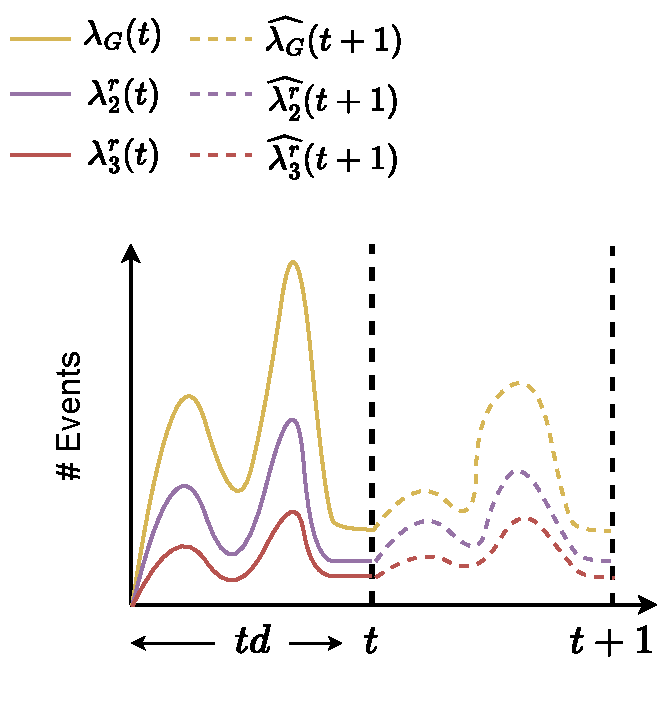
\includegraphics[scale=0.63]{images/concepts/predictive/PA-SPS-Prediction-8.pdf}
\end{figure}
\end{frame}

\begin{frame}{Predictive Approach : PA-SPS}
\begin{figure}
    \centering
    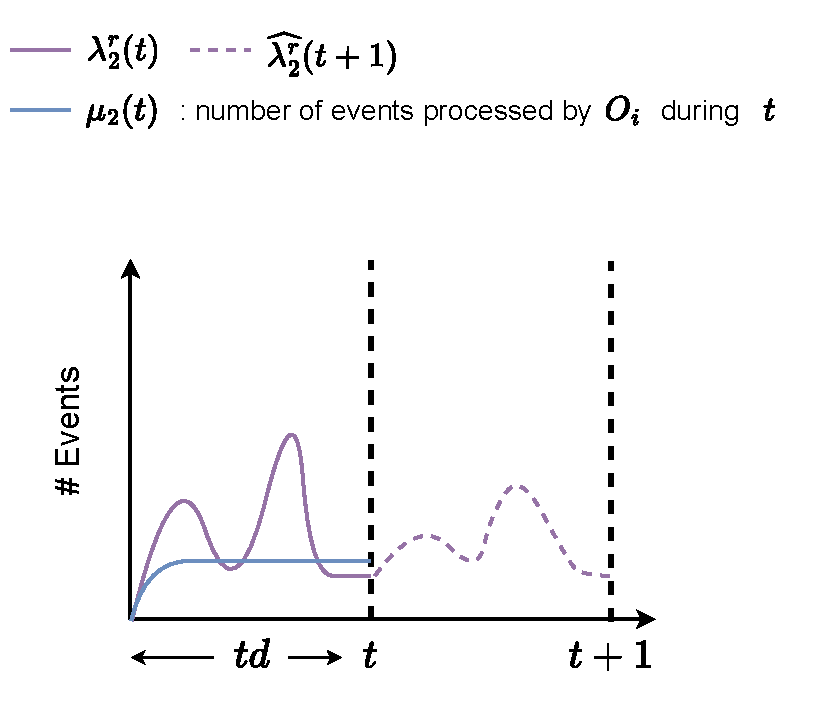
\includegraphics[scale=0.63]{images/concepts/predictive/PA-SPS-Prediction-9.pdf}
\end{figure}
\end{frame}

\begin{frame}{Predictive Approach : PA-SPS}
\begin{figure}
    \centering
    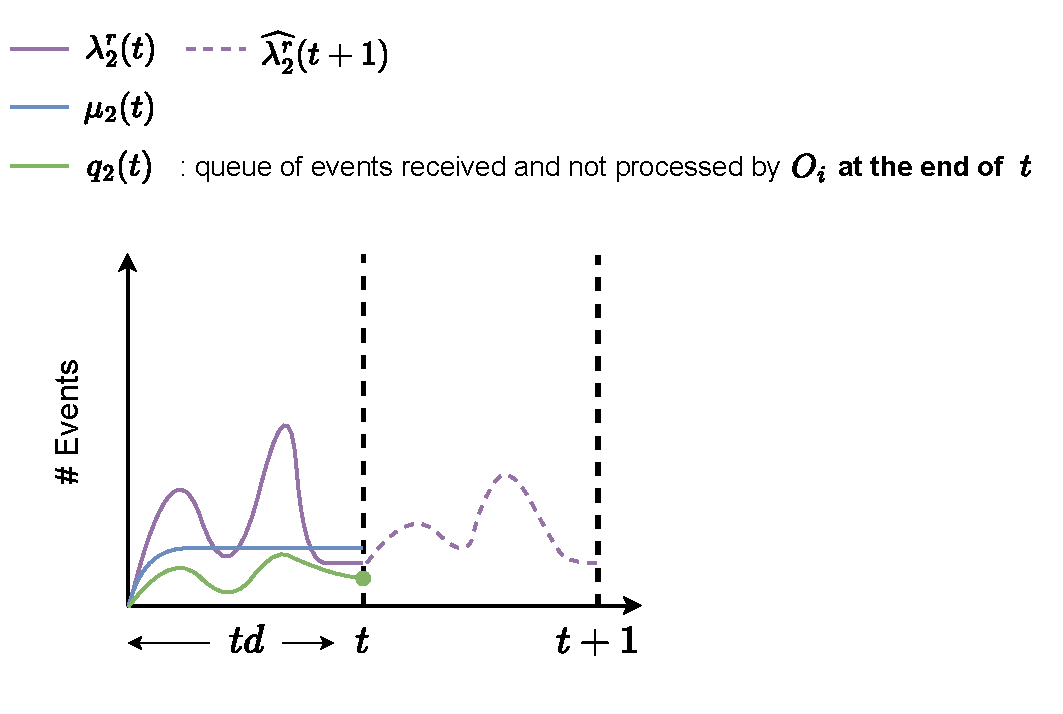
\includegraphics[scale=0.63]{images/concepts/predictive/PA-SPS-Prediction-10.pdf}
\end{figure}
\end{frame}

\begin{frame}{Predictive Approach : PA-SPS}
\begin{figure}
    \centering
    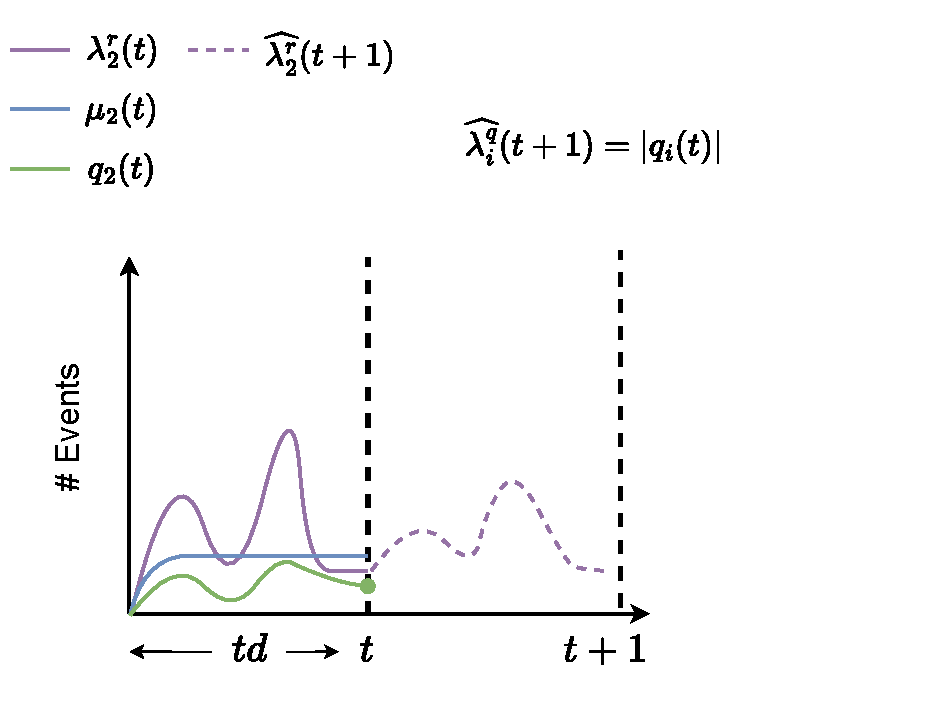
\includegraphics[scale=0.63]{images/concepts/predictive/PA-SPS-Prediction-10-2.pdf}
\end{figure}
\end{frame}

\begin{frame}{Predictive Approach : PA-SPS}
\begin{figure}
    \centering
    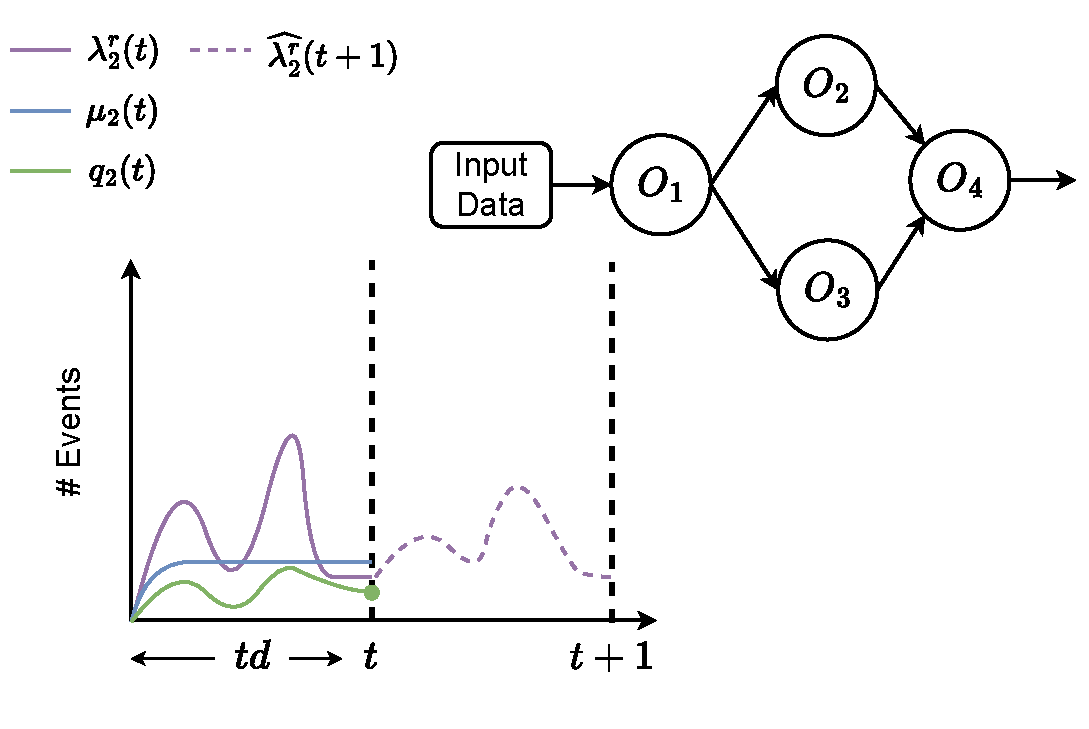
\includegraphics[scale=0.63]{images/concepts/predictive/PA-SPS-Prediction-11.pdf}
\end{figure}
\end{frame}

\begin{frame}{Predictive Approach : PA-SPS}
\begin{figure}
    \centering
    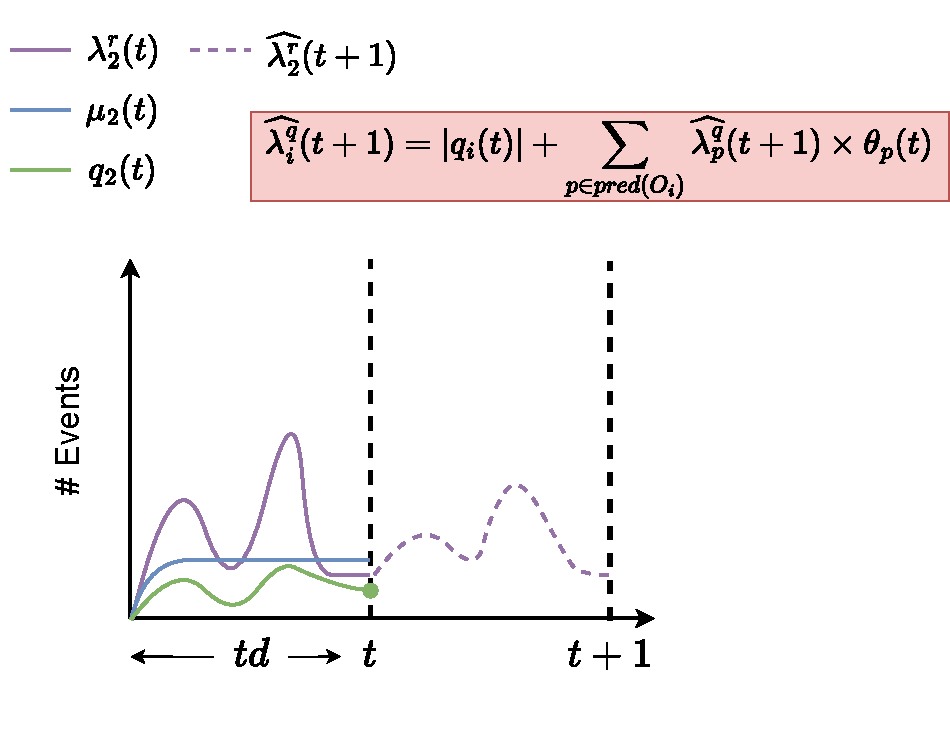
\includegraphics[scale=0.63]{images/concepts/predictive/PA-SPS-Prediction-12.pdf}
\end{figure}
\end{frame}

\begin{frame}{Predictive Approach : PA-SPS}
\begin{figure}
    \centering
    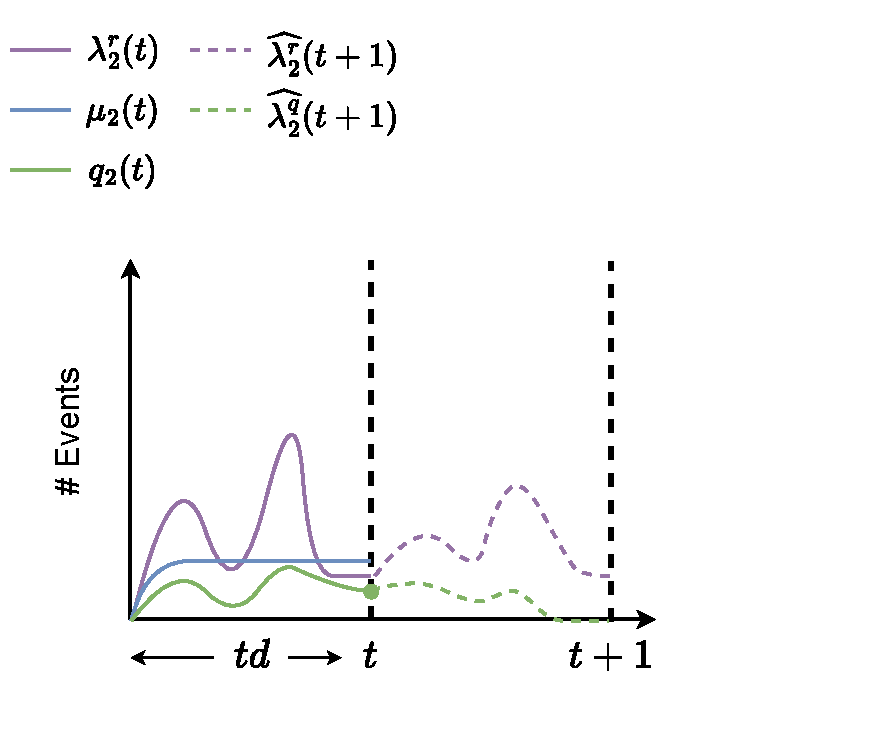
\includegraphics[scale=0.63]{images/concepts/predictive/PA-SPS-Prediction-13.pdf}
\end{figure}
\end{frame}

\begin{frame}{Predictive Approach : PA-SPS}
\begin{figure}
    \centering
    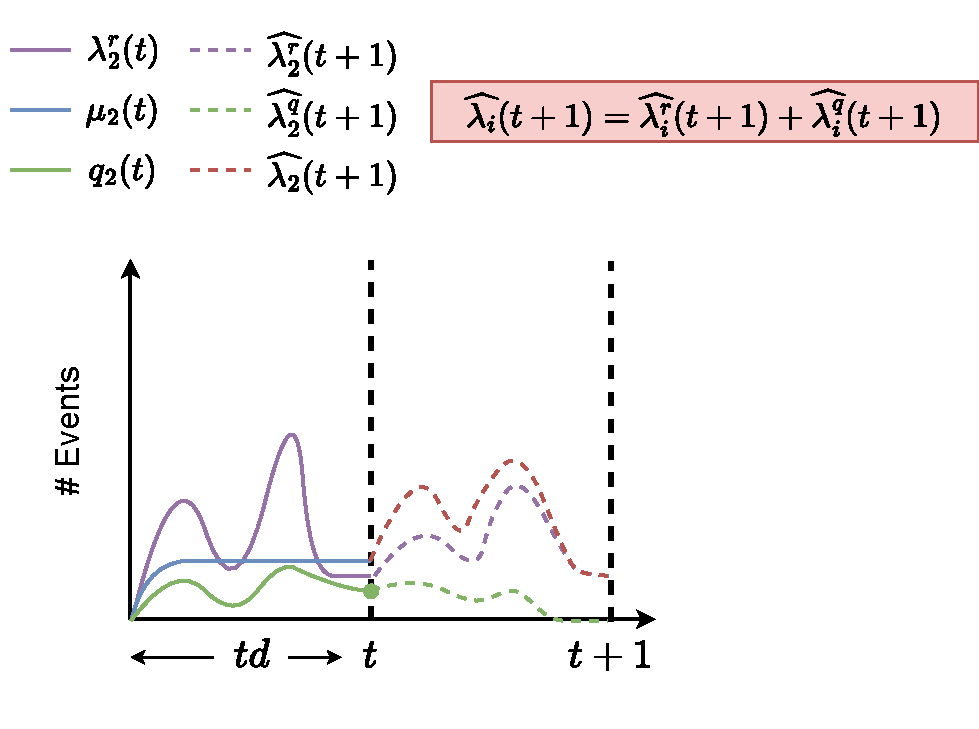
\includegraphics[scale=0.63]{images/concepts/predictive/PA-SPS-Prediction-14.pdf}
\end{figure}
\end{frame}

\begin{frame}{Predictive Approach : PA-SPS}
	\textbf{Prediction of number of active replicas}

	\begin{align*}
		r_i(t+1) = \frac{\widehat{\lambda_i}(t+1) \times et_i}{td}
	\end{align*}
	
%	\begin{tabular}{r l}
%	$r_i(t+1)$ & number of active replicas of operator $Oi$ computed at\\
%			   & the end of $t$\\
%   	$\widehat{\lambda_i}(t+1)$ & predicted number of events to process by operator $O_i$\\
%   	 						   & during $t$ \\
%   	${et}_i$ & average execution time of one event by operator $O_i$ \\
%	$td$ & time interval duration \\
%   	\end{tabular}
\end{frame}

\begin{frame}{PA-SPS : Prediction of active replicas}
	\textbf{Planning algorithm}
	\begin{center}
	\begin{align*}
		r_i(t+1) = \frac{\widehat{\lambda_i}(t+1) \times et_i}{td}
	\end{align*}

    \begin{figure}
    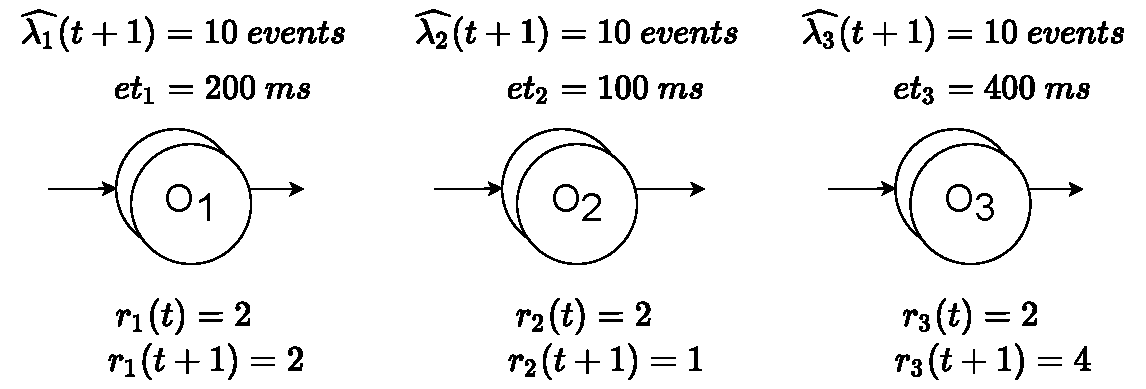
\includegraphics[scale=0.5]{images/concepts/predictive/PA-SPS-PredictiveModel.pdf}
    \end{figure}

    $td = 1000 ms$
   	\end{center}
\end{frame}
\section[4]{Experiments}

\begin{frame}{Environment : Input data scenario}
	A traffic model from real Twitter data related to COVID pandemic

    \begin{figure}[!ht]
        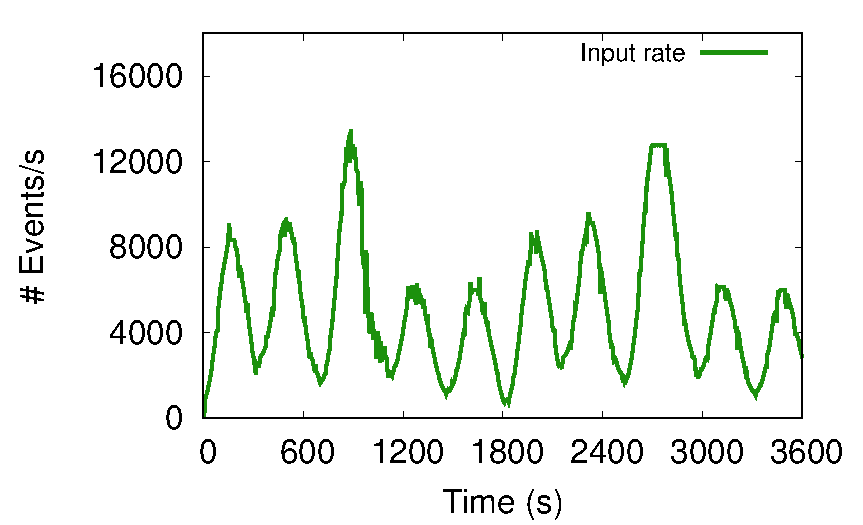
\includegraphics[width=0.75\textwidth]{images/exp/Dataset-TwitterSmoothed.pdf}
        %\caption{Traffic shape of Covid Twitter dataset.}
    \end{figure}
\end{frame}

\begin{frame}{Environment : Application}
	Twitter linear app to classify tweets
	\begin{figure}
		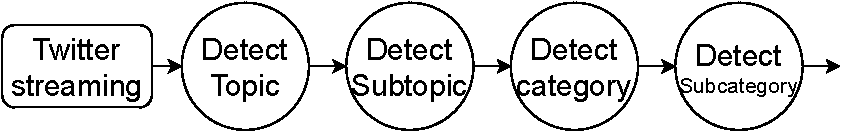
\includegraphics[width=0.9\textwidth]{images/exp/App-Twitter-Linear-1.pdf}
	\end{figure}
\end{frame}

\begin{frame}{Environment : Infrastructure}
	Google Cloud Platform as infrastructure for the deployment

	\begin{figure}
		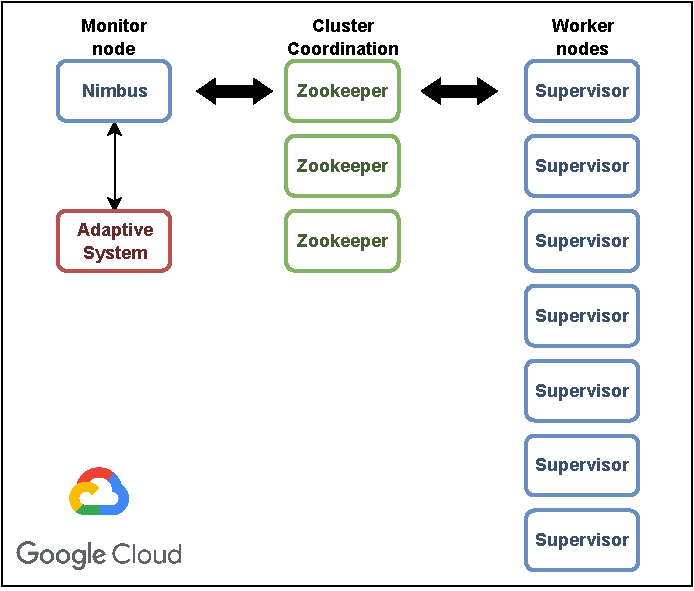
\includegraphics[width=0.75\textwidth]{images/exp/GCP-2.pdf}
	\end{figure}
\end{frame}

\begin{frame}{Evaluation metrics}
	\textit{Saved nodes {\tiny [\cite{LombardiABQ18}]}}
        \begin{itemize}
            \item Proportion
of resources saved with respect to a statically over-provisioned configuration
		 \end{itemize}
	\textit{Throughput degradation {\tiny [\cite{LombardiABQ18}]}}
		 \begin{itemize}
            \item Difference between the input rate and the output rate
         \end{itemize}
	\textit{Latency}
		 \begin{itemize}
         	\item Average time taken by an event between the moment it enters and leaves the SPS
         \end{itemize}
	\textit{Difference in the number of processed events}
		 \begin{itemize}         
            \item Difference between the total number of processed events and the total number of received events
        \end{itemize}
\end{frame}


\begin{frame}[noframenumbering]
	\centering
	\huge Performance Results \\ Reactive approach (RA-SPS)
\end{frame}

\begin{frame}{Performance Results : Reactive approach (RA-SPS)}
	\begin{columns}
	\begin{column}{0.6\textwidth}
    	\begin{figure}
		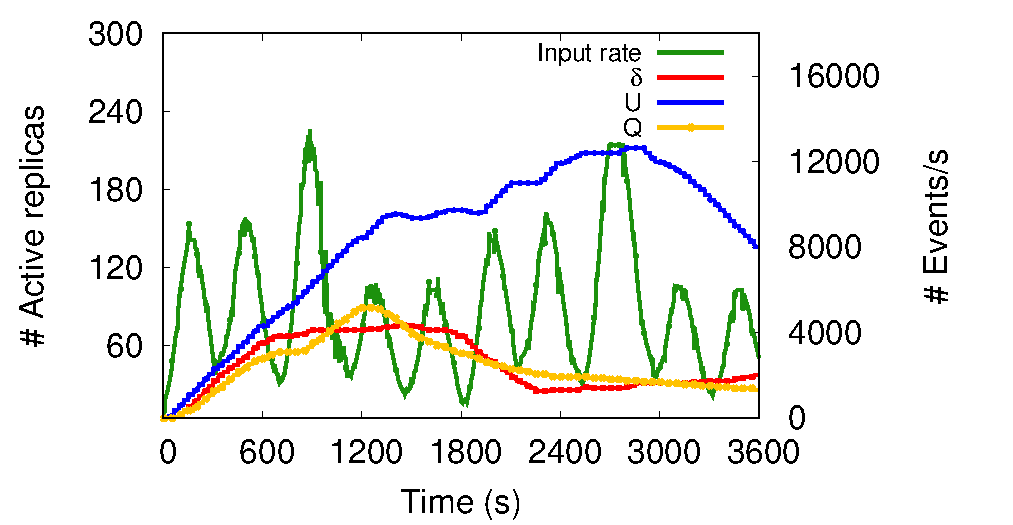
\includegraphics[width=\textwidth]{images/exp/reactive/TwitterLinear-Replicas.pdf}

		\end{figure}
	\end{column}
    \begin{column}{0.55\textwidth}
	    \begin{figure}
		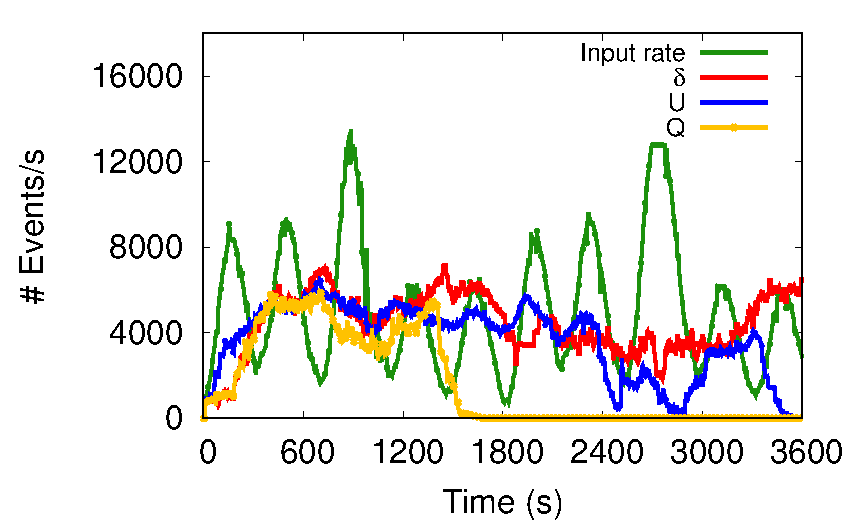
\includegraphics[width=\textwidth]{images/exp/reactive/TwitterLinear-Throughput.pdf}
		\end{figure}
	\end{column}
	\end{columns}
	
	\begin{itemize}
		\item Q queues a lot of events
		\item U overprovides active replicas
		\item $\delta$ is more stable
	\end{itemize}
\end{frame}

\begin{frame}{Performance Results : Reactive approach (RA-SPS)}
	\centering
	
	\begin{table}[!ht]
    \begin{tabular}{|l|llll|}
        \hline
        Metric & \begin{tabular}[c]{@{}l@{}}Saved\\ Nodes\end{tabular} & \begin{tabular}[c]{@{}l@{}}Throughput\\ Degradation\end{tabular} & \begin{tabular}[c]{@{}l@{}}Diff. Proc.\\ Events\end{tabular} & \begin{tabular}[c]{@{}l@{}}Latency\\ (ms)\end{tabular} \\ \hline \hline
        \textbf{$\delta$} & \textbf{0.3996}  & \textbf{0.1092} & \textbf{0.8907} & \textbf{39687.51} \\ \hline
        U        & -0.8934 & 0.2597 & 0.7402 & 23441.39 \\ \hline
        Q        & 0.4975  & 0.6830 & 0.3169 & 28799.60 \\ \hline
        \end{tabular}
    \end{table}
    
    \begin{itemize}
    	\item $\delta$ process more events that U and Q
    	\item $\delta$ does not consider dependency, so there is cascading problem
    \end{itemize}
\end{frame}


\begin{frame}[noframenumbering]
	\centering
	\huge Performance Results \\ Predictive approach (PA-SPS)
\end{frame}

\begin{frame}{Performance Results : Predictive approach (PA-SPS)}	
	\centering

	\begin{table}[!ht]
	\begin{tabular}{|l|llll|}
	\hline \begin{tabular}[c]{@{}l@{}}Pred.\\ Model\end{tabular} & \begin{tabular}[c]{@{}l@{}}Saved\\ Resources\end{tabular} & \begin{tabular}[c]{@{}l@{}}Throughput\\ Degradation\end{tabular} & \begin{tabular}[c]{@{}l@{}}Diff. Proc.\\ Events\end{tabular} & \begin{tabular}[c]{@{}l@{}}Latency\\ (ms)\end{tabular} \\ \hline \hline
	\textbf{ANN}   & \textbf{0.475} & \textbf{0.070} & \textbf{1.000}      & \textbf{355.490}   \\ \hline
	FFT   & 0.519 & 0.189 & 1.000      & 1023.380 \\ \hline
	LR    & 0.533 & 0.195 & 1.000      & 663.030  \\ \hline
	RF    & 0.538 & 0.227 & 0.996      & 583.921   \\ \hline
	Basic & 0.560 & 0.325 & 1.000      & 1295.490  \\ \hline
	\end{tabular}
	\end{table}
	
	\begin{itemize}
		\item ANN has a low latency and is more stable, but use more resource
		\item Trade-off : Resource vs Performance
	\end{itemize}
\end{frame}

%\begin{frame}{Performance Results}
%	\begin{columns}
%    \begin{column}{0.5\textwidth}
%	    \begin{figure}
%		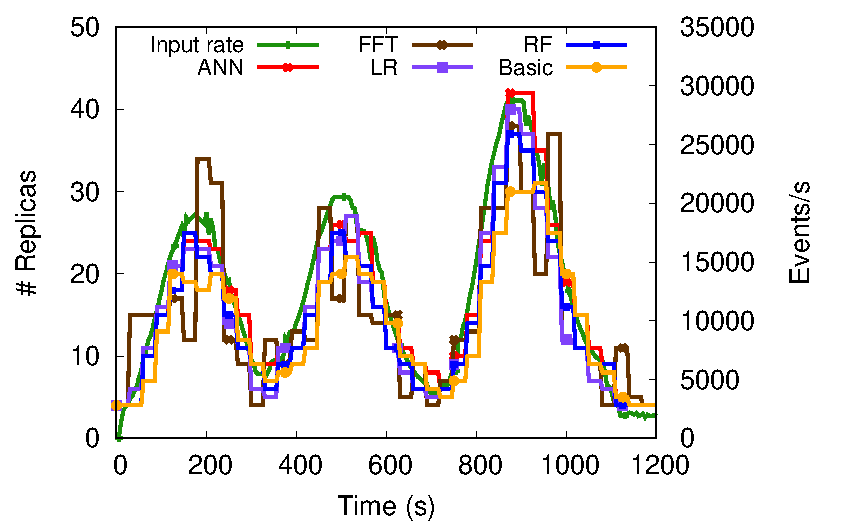
\includegraphics[width=1\textwidth]{images/exp/predictive/TwitterLinear-Models-Replicas.pdf}
%        \caption{Total number of replicas.}
%		\end{figure}
%	\end{column}
%    \begin{column}{0.5\textwidth}
%    	\begin{figure}
%		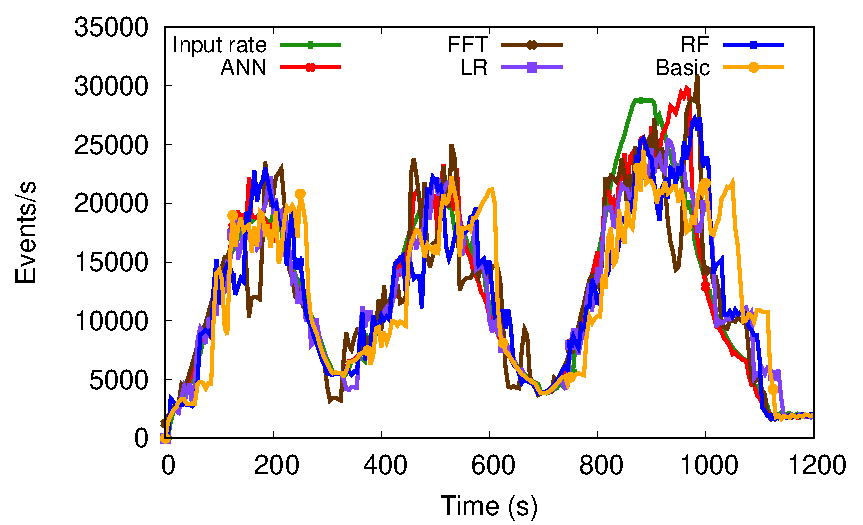
\includegraphics[width=1\textwidth]{images/exp/predictive/TwitterLinear-Models-Throughput.pdf}
%        \caption{Throughput.}
%		\end{figure}
%	\end{column}
%	\end{columns}
%	
%	\begin{center}
%	    Comparison of different models
%	\end{center}
%\end{frame}

\begin{frame}{Performance Results : Predictive approach (PA-SPS)}
	Comparison between PA-SPS and DABS
	\begin{itemize}
		\item PA-SPS : 
		\begin{itemize}
			\item Uses ANN as a predictor model
		\end{itemize}
		\item DABS :
		\begin{itemize}
		 	\item An extension of Storm 
		 	\item Uses a predictor model based on regressions
		\end{itemize}
	\end{itemize}
\end{frame}

\begin{frame}{Performance Results : Predictive approach (PA-SPS)}
	\begin{columns}
    \begin{column}{0.55\textwidth}
    	\centering
	    \begin{figure}
		\includegraphics[width=1\textwidth]{images/exp/predictive/TwitterLinear-RW-Replicas.pdf}
		\end{figure}
	\end{column}
    \begin{column}{0.55\textwidth}
    	\centering
    	\begin{figure}
		\includegraphics[width=1\textwidth]{images/exp/predictive/TwitterLinear-RW-Throughput.pdf}
		\end{figure}
	\end{column}
	\end{columns}
	
	\begin{itemize}
		\item DABS restarts many times the application
		\item PA-SPS is more stable
	\end{itemize}
\end{frame}

\begin{frame}{Performance Results : Predictive approach (PA-SPS)}
	\centering
	\begin{table}[!ht]
        \begin{tabular}{|l|llll|}
            \hline
          \begin{tabular}[c]{@{}l@{}}Adaptive\\ SPS\end{tabular}  & \begin{tabular}[c]{@{}l@{}}Saved\\ Resources\end{tabular} & \begin{tabular}[c]{@{}l@{}}Throughput\\ Degradation\end{tabular} & \begin{tabular}[c]{@{}l@{}}Diff. Processed\\ Events\end{tabular} & \begin{tabular}[c]{@{}l@{}}Latency\\ (ms)\end{tabular} \\ \hline \hline
            PA-SPS     & 0.475   & 0.071 & 1.000 & 355.490   \\ \hline
            DABS    & 0.3962   & 0.2849 & 0.8283 & 1391.28 \\ \hline
        \end{tabular}
    \end{table}
    \begin{itemize}
    	\item DABS has a less efficient adaptation in contrast to PA-SPS
    \end{itemize}
\end{frame}

%\begin{frame}{Performance Results : Predictive approach (PA-SPS)}	
%	\centering
%	\begin{table}[!ht]
%	\begin{tabular}{|l|llll|}
%	\hline Pred. Model & \begin{tabular}[c]{@{}l@{}}Saved\\ Resources\end{tabular} & \begin{tabular}[c]{@{}l@{}}Throughput\\ Degradation\end{tabular} & \begin{tabular}[c]{@{}l@{}}Diff. Proc.\\ Events\end{tabular} & \begin{tabular}[c]{@{}l@{}}Latency\\ (ms)\end{tabular} \\ \hline \hline
%	ANN PA-SPS   & 0.475 & \textbf{0.070} & \textbf{1.000}      & \textbf{355.490}   \\ \hline
%	LR (DABS) PA-SPS    & \textbf{0.533} & 0.195 & \textbf{1.000}      & 663.030  \\ \hline
%	\end{tabular}
%	\end{table}
%	
%	Metric values
%\end{frame}

\section[5]{Conclusion}

\begin{frame}{Conclusion}
\textbf{Adaptive SPS} extending Storm
\begin{itemize}
	\item \textbf{Pool of replicas}
	\item \textbf{Load-aware grouping}
\end{itemize}
	
Two approaches:
\begin{itemize}
	\item \textbf{Reactive (RA-SPS)} : Use of a multi-metric
	\item \textbf{Predictive (PA-SPS)} : Estimate number of active replicas using different predictive models
\end{itemize}
\end{frame}

\begin{frame}{Future work}
Dynamic adaptation of parameters
	\begin{itemize}
		\item RA-SPS uses different parameters, which can be adjusted by AI
	\end{itemize}
	
Hybrid adaptive SPS
	\begin{itemize}
		\item Use the reactive and predictive model for SPS adaptation
	\end{itemize}

Physical and logical adaptation
	\begin{itemize}
		\item Consider also the modification of virtual machines
	\end{itemize}
\end{frame}

\begin{frame}{}

	{\Huge Merci beaucoup !}
\end{frame}

\begin{frame}{Publications}
\footnotesize

\begin{itemize}
	\item[-] [\cite{WladdimiroNCA}] Daniel Wladdimiro, Luciana Arantes, Pierre Sens and Nicolas Hidalgo. "A Multi-Metric Adaptive Stream Processing System." In: NCA. IEEE, 2021.
	\item[-] [\cite{WladdimiroSBAC}] Daniel Wladdimiro, Luciana Arantes, Pierre Sens and Nicolas Hidalgo. "A predictive approach for dynamic replication of operators in distributed stream processing systems" In: SBAC. IEEE, 2022.
	\item[-] [\cite{WladdimiroJPDC}] Daniel Wladdimiro, Luciana Arantes, Pierre Sens and Nicolas Hidalgo. "PA-SPS: A Predictive Adaptive Approach for an Elastic Stream Processing System" In: JPDC. 2023. [Minor Revision]
	\item[-] [\cite{WladdimiroComPAS2022}] Daniel Wladdimiro, Luciana Arantes, Pierre Sens and Nicolas Hidalgo. "A predictive model for Stream Processing System that dynamically calibrates the number of operator replicas." In: ComPAS. Amiens, France, 2022.
	\item[-] [\cite{WladdimiroComPAS2023}] Daniel Wladdimiro, Luciana Arantes, Pierre Sens and Nicolas Hidalgo. "PRESPS: a PREdictive model to determine the number of replicas of the operators in Stream Processing Systems" In: ComPAS. Annecy, France,
2023.
\end{itemize}
\end{frame}



\appendix

\begin{frame}[allowframebreaks]
\frametitle{References}
\printbibliography
\end{frame}

\end{document}

